% !TeX spellcheck = en_GB

% List of packages and options for them
% Base packages
\documentclass[a4paper,10pt]{article}
\usepackage{a4wide} \bibliographystyle{plain}
\usepackage[english]{babel}
\usepackage{parskip} % To prevent indentation of new paragraphs
\usepackage[utf8]{luainputenc}
\usepackage{lmodern} % Modern font with a.o. euro symbols included
\usepackage[T1]{fontenc} % Fix font encoding in the document to improve the layout
\usepackage{placeins} % Barrier for floats
\usepackage{eurosym} % Include the euro symbol
\usepackage{etoolbox}

% Text layout packages
\usepackage{color} % For fancy colors
\usepackage{xcolor} % For colors
\usepackage[hidelinks]{hyperref}
\hypersetup{colorlinks=false,linkbordercolor=gray!30!white,pdfborderstyle={/S/U/W 1}}
\usepackage[inline]{enumitem} % For lists
\usepackage{fontspec} % For custom fonts
\usepackage{microtype} % For better text appearance
\usepackage{soul} % For strikethrough text

% Figures & References packages
\usepackage[labelfont=bf]{caption} \captionsetup{width=0.8\linewidth, font=small} % For captions
\usepackage{subcaption} % For more advanced captions, such as figure 1a, b, c
\usepackage{wrapfig} % For figures on the side of the text
%\usepackage{epstopdf} % To be able to include eps files
%\usepackage{graphicx} % Include more types of images
\usepackage{elasticrow}

% Graphs packages
\usepackage{tikz} % Used for custom vectors and other drawings
\usepackage{tikzscale}
\usetikzlibrary{external} \tikzexternalize[prefix=_tikz-cache/] \tikzsetfigurename{reference_} % Cached tikz graphics
\usepackage{pgfplots} \usepgfplotslibrary{fillbetween,patchplots,groupplots,polar} \pgfplotsset{compat=newest} % For fancy graphs
\usepackage{pgfplotstable} % To use tables as data source for graphs
\usepackage{filecontents} % To export content to a given file from latex outside the preamble
\usepackage{scaletikz}

% Positioned here for compatibility with tikz externalize
\usepackage[xindy,toc]{glossaries} % For glossaries

% Table packages
\usepackage{booktabs} % Used for lines in tables
\usepackage{array} % For vertical alignment of text in cells
\usepackage{xltabular} % For page-spanning tables
\usepackage{multirow} % For row-spans besides column-spans
\usepackage[column=C]{cellspace} \addparagraphcolumntypes{X} % Tables with paragraph columns

% Fix normal tabular booktabs
\AtBeginEnvironment{tabular}{\let\xltabular\undefined}
\AtBeginEnvironment{tabularx}{\let\xltabular\undefined}

% Computing Science packages
\usepackage{listings} % For code listings
\usepackage{minted} % For code coloring (requires color)

% Maths packages
\usepackage{amsmath} % For most maths things
\usepackage{physics} % For derivative sign things
\usepackage{mathtools} % More maths things (fixes things in amsmath, requires it as well)
\usepackage{amssymb} % Special symbols

% Physics packages
\usepackage{siunitx} \sisetup{separate-uncertainty=true, exponent-product=\cdot} % Si units!

% Coding setup
\definecolor{Gray}{gray}{0.95}

\defaultfontfeatures{RawFeature={+axis={wght=100}}}
\setmonofont[Scale=0.88,RawFeature={+axis={wght=350}}]{CascadiaMono.ttf}
\newfontface\ttbf{CascadiaMono.ttf}[Scale=0.88,RawFeature={+axis={wght=700}}]
\renewcommand{\theFancyVerbLine}{\sffamily\textcolor[rgb]{0.5,0.5,0.5}{\scriptsize\arabic{FancyVerbLine}}}
\renewcommand{\listingscaption}{Code sample}

\usemintedstyle{vs}
\usemintedstyle[TeX]{lovelace}
\usemintedstyle[gnuplot]{lovelace}

\newminted[texlong]{TeX}{
	linenos,
	frame=lines,
	framesep=3mm,
	breaklines,
	breakautoindent=true,
	fontsize = \fontsize{8pt}{10.5pt},
	tabsize = 4,
	bgcolor=white
}

\newminted[texs]{TeX}{
	tabsize = 4,
	breaklines,
	breakautoindent=true,
	bgcolor=white
}

\newminted[gnuplots]{gnuplot}{
	tabsize = 4,
	breaklines,
	breakautoindent=true,
	bgcolor=white
}

\newmintinline[tex]{TeX}{
	mathescape,
	tabsize = 4
}

\newmintinline[gnup]{gnuplot}{
	mathescape,
	tabsize = 4
}

% Document info
\title{LaTeX Reference}
\author{Floris Westerman}

% Leaders
\newcommand*{\titlerule}[3][]{%
  \makebox[#2]{#1%
    \leaders\hrule height \dimexpr.5ex+.2pt\relax depth \dimexpr-.5ex+.2pt\relax \hfill% Left rule
    \enskip{#3}\enskip% Text (and surrounding spaces)
    \leaders\hrule height \dimexpr.5ex+.2pt\relax depth \dimexpr-.5ex+.2pt\relax \hfill\kern0pt}% Right rule
	\vspace{3pt}
}

% Middle of text comment
\newcommand{\comment}[2]{%
	\vspace{6pt}
	\makebox[\linewidth][c]{%
		\begin{minipage}{.9\linewidth}
			\titlerule{\linewidth}{\footnotesize\bf#1}
			#2
			\vspace{8pt}\hrule
		\end{minipage}
	}
	\vspace{6pt}
}

% Better vectors in latex
\makeatletter
\newlength\xvec@height%
\newlength\xvec@depth%
\newlength\xvec@width%
\newcommand{\xvec}[2][]{%
	\ifmmode%
	\settoheight{\xvec@height}{$#2$}%
	\settodepth{\xvec@depth}{$#2$}%
	\settowidth{\xvec@width}{$#2$}%
	\else%
	\settoheight{\xvec@height}{#2}%
	\settodepth{\xvec@depth}{#2}%
	\settowidth{\xvec@width}{#2}%
	\fi%
	\def\xvec@arg{#1}%
	\def\xvec@dd{:}%
	\def\xvec@d{.}%
	\raisebox{.2ex}{\raisebox{\xvec@height}{\rlap{%
		\kern.05em%  (Because left edge of drawing is at .05em)
		\tikzset{external/export=false}%
		\begin{tikzpicture}[scale=1]
		\pgfsetroundcap
		\draw (.05em,0)--(\xvec@width-.05em,0);
		\draw (\xvec@width-.05em,0)--(\xvec@width-.15em, .075em);
		\draw (\xvec@width-.05em,0)--(\xvec@width-.15em,-.075em);
		\ifx\xvec@arg\xvec@d%
		\fill(\xvec@width*.45,.5ex) circle (.5pt);%
		\else\ifx\xvec@arg\xvec@dd%
		\fill(\xvec@width*.30,.5ex) circle (.5pt);%
		\fill(\xvec@width*.65,.5ex) circle (.5pt);%
		\fi\fi%
		\end{tikzpicture}%
	}}}%
	#2%
}
\makeatother

% --- Override \vec with an invocation of \xvec.
\let\stdvec\vec
\renewcommand{\vec}[1]{\xvec[]{#1}}
% --- Define \dvec and \ddvec for dotted and double-dotted vectors.
\newcommand{\dvec}[1]{\xvec[.]{#1}}
\newcommand{\ddvec}[1]{\xvec[:]{#1}}
\newcommand{\iu}{{i\mkern1mu}}

% Some sizing hack
\newsavebox{\measuredSize}
\newcommand{\resizeToWidth}[2]{%
	\pgfmathsetmacro{\pgfplotswidth}{#2}%
	\begin{lrbox}{\measuredSize}#1\end{lrbox}%
	\pgfmathsetmacro{\pgfplotswidth}{2*\pgfplotswidth-\wd\measuredSize}%
	#1%
}

% Requires thing
\usepackage{xparse}
\NewDocumentCommand\requires{mgg}{%
	{\bf\footnotesize This requires the {\tt #1} package\IfNoValueTF{#2}{}{ with the {\tt #2} option}\IfNoValueTF{#3}{\par}{#3}}
}

\def\arraystretch{1.4}

% Glossaries
\newglossarystyle{packages}{%
  \renewenvironment{theglossary}%
    {\begin{longtable}{lp{.6\linewidth}>{\raggedright}p{.1\linewidth}}}%
    {\end{longtable}}%
  \renewcommand*{\glossaryheader}{}%
  \renewcommand*{\glsgroupheading}[1]{}%
  \renewcommand{\glossentry}[2]{%
    \glsentryitem{##1}\glstarget{##1}{\glossentryname{##1}} &
    \glossentrydesc{##1} & ##2\tabularnewline
  }%
  \renewcommand{\subglossentry}[3]{%
     &
     \glssubentryitem{##2}%
     \glstarget{##2}{\strut}\glossentrydesc{##2} &
     ##3\tabularnewline
  }%
  \ifglsnogroupskip
    \renewcommand*{\glsgroupskip}{}%
  \else
    \renewcommand*{\glsgroupskip}{ & & \tabularnewline}%
  \fi
}
% PACKAGE LIST
\makeglossaries
\newglossaryentry{enumitem}
{
	name={\tt enumitem},
	description={Extends customizability of lists},
	sort=enumitem
}
\newglossaryentry{a4wide}
{
	name={\tt a4wide},
	description={Makes the text width in the article document class wider},
	sort=a4wide
}
\newglossaryentry{parskip}
{
	name={\tt parskip},
	description={Removes the indentation in the first line of a new paragraph},
	sort=parskip
}
\newglossaryentry{placeins}
{
	name={\tt placeins},
	description={Provides the possibility to force all floating objects to be printed before continuing},
	sort=placeins
}
\newglossaryentry{pdfpages}
{
	name={\tt pdfpages},
	description={Allows pdfs to be included in your tex document},
	sort=pdfpages
}
\newglossaryentry{eurosym}
{
	name={\tt eurosym},
	description={Includes the euro symbol},
	sort=eurosym
}
\newglossaryentry{hyperref}
{
	name={\tt hyperref},
	description={Adds possibility to add URLs in your document and makes references clickable},
	sort=hyperref
}
\newglossaryentry{color}
{
	name={\tt color},
	description={Adds coloring options for your text},
	sort=color
}
\newglossaryentry{multicol}
{
	name={\tt multicol},
	description={Separates your text into several columns},
	sort=multicol
}
\newglossaryentry{fontspec}
{
	name={\tt fontspec},
	description={Allows the use of custom fonts},
	sort=fontspec
}
\newglossaryentry{soul}
{
	name={\tt soul},
	description={Allows for strike-through text},
	sort=soul
}
\newglossaryentry{caption}
{
	name={\tt caption},
	description={Makes captions more advanced and customizable},
	sort=caption
}
\newglossaryentry{subcaption}
{
	name={\tt subcaption},
	description={Adds the possibility to use subfigures and -captions},
	sort=subcaption
}
\newglossaryentry{wrapfig}
{
	name={\tt wrapfig},
	description={Allows figures to be placed next to text such that text wraps around it},
	sort=wrapfig
}
\newglossaryentry{epstopdf}
{
	name={\tt epstopdf},
	description={Converts {\tt .eps} files to {\tt .pdf} files to be included in your document},
	sort=epstopdf
}
\newglossaryentry{graphicx}
{
	name={\tt graphicx},
	description={Allows to include pictures into your document},
	sort=graphicx
}
\newglossaryentry{tikz}
{
	name={\tt tikz},
	description={Used for vector-based drawings in \LaTeX},
	sort=tikz
}
\newglossaryentry{pgfplots}
{
	name={\tt pgfplots},
	description={Used to create and generate graphs. Requires \gls{tikz}},
	sort=pgfplots
}
\newglossaryentry{pgfplotstable}
{
	name={\tt pgfplotstable},
	description={Allows the use of data files for graphs in {\gls{pgfplots}}},
	sort=pgfplotstable
}
\newglossaryentry{filecontents}
{
	name={\tt filecontents},
	description={Makes it possible to create external files inside \LaTeX},
	sort=filecontents
}
\newglossaryentry{booktabs}
{
	name={\tt booktabs},
	description={Adds better lines for inside tables},
	sort=booktabs
}
\newglossaryentry{array}
{
	name={\tt array},
	description={Allows for custom vertical alignment of content inside table cells},
	sort=array
}
\newglossaryentry{longtable}
{
	name={\tt longtable},
	description={Allows tables to span multiple pages},
	sort=longtable
}
\newglossaryentry{multirow}
{
	name={\tt multirow},
	description={Enables cells to span multiple rows as well besides just multiple columns},
	sort=multirow
}
\newglossaryentry{listings}
{
	name={\tt listings},
	description={Adds an environment to put programming code in. See also \gls{minted} for highlighting},
	sort=listings
}
\newglossaryentry{minted}
{
	name={\tt minted},
	description={Automatically highlights programming code},
	sort=minted
}
\newglossaryentry{amsmath}
{
	name={\tt amsmath},
	description={Adds a lot of symbols and functionality for inside a maths environment},
	sort=amsmath
}
\newglossaryentry{mathtools}
{
	name={\tt mathtools},
	description={Fixes some problems in \gls{amsmath} and extends it},
	sort=mathtools
}
\newglossaryentry{physics}
{
	name={\tt physics},
	description={Adds a lot of shorthand-notation for often-used mathematical expressions in physics},
	sort=physics
}
\newglossaryentry{amssymb}
{
	name={\tt amssymb},
	description={Adds many mathematical symbols to be used},
	sort=amssymb
}
\newglossaryentry{mathdots}
{
	name={\tt mathdots},
	description={Provides many more kinds of dots in the mathematics environment},
	sort=mathdots
}
\newglossaryentry{siunitx}
{
	name={\tt siunitx},
	description={Provides excellent number- and unit formatting capabilities},
	sort=siunitx
}
\newglossaryentry{mhchem}
{
	name={\tt mhchem},
	description={Enables you to write chemical equations and structural diagrams of molecules},
	sort=mhchem
}
\newglossaryentry{float}
{
	name={\tt float},
	description={Enables you to place your floating environments more precisely},
	sort=float
}
\newglossaryentry{floatrow}
{
	name={\tt floatrow},
	description={Enables you to align multiple floating elements on one line easily},
	sort=floatrow
}

\begin{document}
\maketitle

This document is meant as a reference for basic \LaTeX\ functionality. It should be sufficient to write basic reports and documents for the first years of your study. I the first chapter, the basic workings of \LaTeX\ will be explained and I will guide you on starting to use it. After that, the basics of text formatting and mathematics will be discussed. Later on, more advanced subjects such as tables, matrices, figures and graphs are listed. In the appendix, some more complicated and involved examples are given that can be used as templates for your own document.

In the documents, a lot of packages are mentioned. Each mention of a package is clickable and will lead you to the list of packages that I mentioned or recommend. There, you can also find other places where the packages are mentioned. If you want to know more about some packages, simply Google `CTAN [name]' and you'll easily find the documentation of the package for further reference.

In this document, I often mention the syntax of commands. Such a syntax may look like \tex!\command[<options>]{<name>}!. Here, parts between {\tt <>} are variable parts that you have to fill in yourself; a description is given of what should be put in. These {\tt <>} should be omitted in your final code, the rest of the code should be exactly as it was given.

I plan to extend this document over time with more sections, such as making code listings and doing some chemistry. Therefore, when sharing the document, please share the link and not the pdf itself you will always get the latest version. The latest version can always be downloaded from \underline{\url{https://floriswesterman.nl/LaTeXReference.pdf}}.

For any comments and remarks or if you've found a mistake, please contact me at \newline \underline{\href{mailto:me@floriswesterman.nl}{me@floriswesterman.nl}}.

\newpage
\tableofcontents

%%%%%%%%%%%%%%%%%%%%%%%%%%%%%%%%%%%%%%%%%%%%%%%
%% Basics %%%%%%%%%%%%%%%%%%%%%%%%%%%%%%%%%%%%%
%%%%%%%%%%%%%%%%%%%%%%%%%%%%%%%%%%%%%%%%%%%%%%%

\newpage
\section{Setting up}
Before you can start using \LaTeX\ there are some things to set up, install and configure. Also you'll need some basic content in your document before you can start actually adding your text.

\subsection{Installation}
\subsubsection{Windows, Linux, OS X}
There are multiple ways to compile {\tt .tex} files into {\tt pdf}'s. On all common platforms (Windows, Linux, OS X) it is easiest to install \underline{\href{https://miktex.org/download}{MiKTeX}} as your distribution manager - the program that manages all packages and other prerequisites to use \LaTeX.

MiKTeX also already includes a very basic editor. For more advanced functionality, such as code completion, highlighting and others, there are multiple editors available. I'd advise using \underline{\href{https://www.texstudio.org/}{TeXstudio}}, a versatile editor that features a lot of functionality and other options.

For OS X there is also \underline{\href{https://www.texpad.com/}{TeXpad}}, that integrates both the distribution manager and the editor in one very nice program. One disadvantage is that this software is paid and will cost you around \euro 23.

\subsubsection{Online}
It is also possible to work with \LaTeX\ online. This saves you the trouble of installing programs on your computer and enables you to collaborate directly with others; it works like Google Docs so you can work on documents simultaneously. The main disadvantage is that these websites are generally quite slow to work with, building is often very slow with larger documents taking up to a minute to compile and of course it's required to have an internet connection. Commonly used websites are \underline{\href{https://www.overleaf.com/}{Overleaf}} and \underline{\href{https://www.sharelatex.com/}{ShareLaTeX}}.

\subsection{Structure of a \LaTeX\ document}
\subsubsection{Document class}
A \LaTeX\ document has a general style and set-up. Firstly, each document has a {\tt documentclass} set, a set of basic styles and commands available. Commonly used styles are {\tt book}, {\tt article} and {\tt letter}. These all have their own default font sizes, whitespace sizes, etc. You can also download one of the many styles available on the internet, some specifically designed to make resum\'es, articles for specific scientific journals and many more.

A document class is set using the command \tex!\documentclass[<options>]{<name>}! where your options are specific options for your document class. The options available differ for each class, but you can generally set the paper and font size you're working with. In between the curly brackets you put the name of the document class. This is a common pattern in \LaTeX, options are generally placed in between square brackets in front or after the curly brackets with the actual content.

\subsubsection{Packages}
After that, you'll generally define the packages to be loaded. Packages are the add-ons for \LaTeX, you can add a lot of functionality with them. They enable you to go past the standard feature set of \LaTeX\ and make beautiful graphs, tables and lists. You can make your text {\color{red} more colorful} or change the size of anything you want. When working with MiKTeX, these packages will be downloaded the first time you use them, after that they're permanently loaded.

Packages can be included using the \tex!\usepackage[<options>]{<name>}! command. Again, within the square brackets you can put your options and in between the curly brackets you put the name of the package. In this document I'll sometimes state that some command requires some package or some option, this is how you do that.

\subsubsection{Environments}
All of the above together is called your \emph{preamble}. After this will be the main content of your document. This content is divided into so-called \emph{environments}, `blocks' of content with a specific purpose. Environments are opened, or started, by \tex!\begin{<environment>}! and ended by \tex!\end{<environment>}! where {\tt environment} is the name of your environment. The content in between both statements will be inside that environment. The main environment is {\tt document}, it conatins all content of your document. There are separate environments for maths, your abstract, figures, tables, graphs, lists, etc.

\subsubsection{Example document}
Below is an example of a simple document in \LaTeX. It'll make a document with document class {\tt article} and consist of a title (the commands \tex!\title{}!, \tex!\author{}! and \tex!\maketitle! are defined in the document class) and a short text.

\begin{texlong*}{label=\textrm{Simple \LaTeX\ document},escapeinside=||}
\documentclass[a4paper,10pt]{article}

\usepackage{a4wide}

\title{My fancy report}
\author{Floris Westerman}

\begin{document}
	\maketitle
	This is a nice document
||\end{document}
\end{texlong*}

%%%%%%%%%%%%%%%%%%%%%%%%%%%%%%%%%%%%%%%%%%%%%%%
%% Text things %%%%%%%%%%%%%%%%%%%%%%%%%%%%%%%%
%%%%%%%%%%%%%%%%%%%%%%%%%%%%%%%%%%%%%%%%%%%%%%%

\newpage
\section{Text formatting}
\subsection{Titling}
Titling can be done using the \tex=\section=, \tex=\subsection= and \tex=\subsubsection= commands. Each `sub' indicates a level in your headers. All of them will be included in the table of contents (\tex=\tableofcontents=). There are multiple versions:

\vspace{5pt}
\begin{tabular}{m{.47\textwidth}m{.47\textwidth}}\toprule
\bf Command & \bf Description \\\midrule
\tex=\section{Title}= & Just a normal section. \\
\tex=\section[Short title]{Very long title}= & The short title in between {\tt []} will be put in the table of contents, the long title will be shown in the document itself. \\
\tex=\section*{Title}= & An unnumbered section title. Useful for when there is no ToC or when it is not relevant to have numbering (in a smaller document). \\
\tex=\subsection=, \tex=\subsubsection=, \tex=\paragraph=, \tex=\subparagraph= & Same as above, same options, but lower level and smaller size \\\bottomrule
\end{tabular}

\subsection{Text sizes}
It is possible to write text in {\small smaller} and {\large larger} font sizes. The following font sizes are available:

\vspace{5pt}
\begin{tabular}{m{.37\textwidth}m{.57\textwidth}}\toprule
\bf Command & \bf Description \\\midrule
\tex={\tiny Text}= & This is {\tiny tiny text}. \\
\tex={\scriptsize Text}= & This is {\scriptsize (super-/sub)script sized text}. \\
\tex={\footnotesize Text}= & This is {\footnotesize footnote sized text}. \\
\tex={\small Text}= & This is {\small small text}. \\
\tex={\large Text}= & This is {\large large text}. \\
\tex={\Large Text}= & This is {\Large larger text}. \\
\tex={\LARGE Text}= & This is {\LARGE very large text}. \\
\tex={\huge Text}= & This is {\huge huge text}. \\
\tex={\Huge Text}= & This is {\Huge truly huge text}. \\
\bottomrule
\end{tabular}

\begin{minipage}{\textwidth}
\subsection{Text styles}
There are multiple text styles, such as underlines, italics, etc. You can also change your font size. These commands are available:

\vspace{10pt}
\begin{tabular}{m{.37\textwidth}m{.57\textwidth}}\toprule
\bf Command & \bf Description \\\midrule
\tex=\textbf{Text}= \newline \tex={\bf Text}= & This text will be made {\bf boldface}. \\
\tex=\textit{Text}= \newline \tex={\it Text}= & This text will be made {\it italics}. \\
\tex=\textsl{Text}= \newline \tex={\sl Text}= & This text will be made {\sl slanted}. \\
\tex=\textsc{Text}= \newline \tex={\sc Text}= & This text will be made {\sc small caps}. \\
\tex=\textsf{Text}= \newline \tex={\sf Text}= & This text will be made {\sf Sans Serif}.\\
\tex=\texttt{Text}= \newline \tex={\tt Text}= & This text will be made {\tt monospaced}.\\
\tex=\textsuperscript{Text}= & This text will be made \textsuperscript{superscript}.\\
\tex=\textsubscript{Text}= & This text will be made \textsubscript{subscript}.\\
\tex={\color{blue} Text}={\color{red}*} & This text will be made {\color{blue} blue}.\\
\tex=\underline{Text}= & This text will be made \underline{underlined}.\\
\tex=\st{Text}={\color{red}**} & This text will be made \st{strike-through}.\\
\midrule \multicolumn{2}{l}{{\color{red}*} \requires{\gls{color}}} \\
\midrule \multicolumn{2}{l}{{\color{red}**} \requires{\gls{soul}}} \\
\bottomrule
\end{tabular}
\end{minipage}

\subsection{Paragraphs and alignment}
New paragraphs can simply be introduced using a double enter. If you want to force an `enter' without introducing a new paragraph, one can use the double backslash \tex=\\=. Furthermore, text can be justified left and right and can be centered.

\begin{tabular}{m{.37\textwidth}m{.57\textwidth}}\toprule
\bf Command & \bf Description \\\midrule
\tex=\begin{flushleft}= \newline \tex=    Content=\newline \tex=\end{flushleft}= & This text will be aligned on the left-hand side of the page. \\
\tex=\begin{flushright}= \newline \tex=    Content=\newline \tex=\end{flushright}= & This text will be aligned on the right-hand side of the page. \\
\tex=\begin{center}= \newline \tex=    Content=\newline \tex=\end{center}= & This text will be centered on the page. \\
\tex=\\= \newline \tex=\newline= & This forces a new line to be created. \\
Double enter \newline \tex=\par= & This will create a new paragraph. \\
\tex=\newpage= & This will force a pagebreak, so text will continue on the next page. \\
\bottomrule
\end{tabular}

By default, new paragraphs are indented on the first line. This is the standard in many reports and articles. However, you might not like it. The easiest solution is to simply include the package \gls{parskip}, so put \tex!\usepackage{parskip}! in your preamble.

\subsection{Lists}
\begin{minipage}{\textwidth}
It is possible to make lists with numbers and without numbers. The `counted' lists use the environment {\tt enumerate} and the others use {\tt itemize}. It is also possible to nest multiple lists, so a basic example would be:

\vspace{10pt}
\begin{tabular}{p{.47\textwidth}m{.47\textwidth}}\toprule
\begin{minipage}[c]{\linewidth}
\begin{texs}
\begin{enumerate}
	\item First item
	\item Some sublist:
		\begin{itemize}
			\item Subitem
			\item Subitem
		\end{itemize}
	\item Last item
\end{itemize}
\end{texs}
\end{minipage}%
&
\begin{enumerate}
	\item First item
	\item Some sublist:
		\begin{itemize}
			\item Subitem
			\item Subitem
		\end{itemize}
	\item Last item
\end{enumerate}
\\\bottomrule\end{tabular}
\end{minipage}
\vspace{2pt}

Using the package \gls{enumitem} it is also possible to do some more advanced things. The most useful thing is to define custom labels for your items. You can do roman or letter-notation instead of normal digits and use other shapes in the itemize or even make a sort-of key-value table. Short overview:

\vspace{5pt}
\begin{tabular}{m{.57\textwidth}m{.38\textwidth} @{}}\toprule
\bf Command & \bf Example \\\midrule
\tex!\item [Custom] And the text!
&
\begin{enumerate}[topsep=5pt]\item First \item [Custom] And the text! \item Third\end{enumerate}\vspace*{-\baselineskip}\hspace{0pt} \\
%
%
\tex!\begin{enumerate}[label=\alph*)]!{\color{red}*} & \begin{enumerate}[label=\alph*),topsep=5pt] \item First \item Second\end{enumerate}\vspace*{-\baselineskip}\hspace{0pt} \\
%
%
\tex!\begin{enumerate}[label=\roman*)]!{\color{red}*} & \begin{enumerate}[label=\roman*),topsep=5pt] \item First \item Second\end{enumerate}\vspace*{-\baselineskip}\hspace{0pt} \\
%
%
\tex!\begin{enumerate}[label=\arabic*)]!{\color{red}*} & \begin{enumerate}[label=\arabic*),topsep=5pt] \item First \item Second\end{enumerate}\vspace*{-\baselineskip}\hspace{0pt} \\
%
%
\tex!\begin{enumerate*}[label=\bf(\alph*)]!{\color{red}**} & Inline list: \begin{enumerate*}[label=\bf(\alph*),topsep=5pt]\item first \item second\end{enumerate*}. \\
\midrule \multicolumn{2}{l}{{\color{red}*} \requires{\gls{enumitem}}} \\
\midrule \multicolumn{2}{l}{{\color{red}**} \requires{\gls{enumitem}}{inline}} \\
\bottomrule
\end{tabular}
\vspace{5pt}

The labels \tex!\alph*!, \tex!\roman*! and \tex!\arabic*! are defined in the \gls{enumitem} package. For {\tt itemize} it is possible to use any symbol from any library as label of a list item.

\subsection{References}\label{sec:references}
It is very easy to do references in \LaTeX. With just two lines of code you can refer to any figure, table, section or equation in your document and the numbering will automatically be correct. You just place a \tex!\label{<name>}! command close to whatever you want to refer to and you put \tex!\ref{<name>}! at the place you want to put a reference. Here, {\tt name} is a shorthand name of what you're referring to. In larger documents it can get difficult to distinguish equations from figures from tables, it is common to prefix your names with things like {\tt ch:} for chapters, {\tt fig:} for figures and {\tt eq:} for equations. As an example:

\vspace{5pt}
\begin{tabular}{p{.47\textwidth}m{.47\textwidth}}\toprule
\begin{minipage}{\linewidth}
\begin{texs}
\begin{equation}
	\label{eq:einstein}
	E = mc^2
\end{equation}

(..)

As we saw in equation \ref{eq:einstein}, we have that ...
\end{texs}
\end{minipage}
&
\begin{equation}\label{eq:refsample} E = mc^2 \end{equation}\newline
As we saw in equation \ref{eq:refsample}, we have that ...
\\\bottomrule\end{tabular}\vspace{10pt}

It is also possible to use the command \tex!\pageref{<name>}! that will print the page number the reference is on. Especially for equations, the \gls{amsmath} package has define \tex!\eqref{<name>}! that prints the number with parentheses around it to easily distinguish it from other references without putting `formula' or `equation' in your text all the time.

In longer documents it is also useful to include the section number in your numbering and reset your numbering with each new section. This will prevent your numbers from getting too high and it makes it more convenient to look up the references in the document. Again, \gls{amsmath} has a nice command for this: use \tex!\numberwithin{<countera>}{<counterb>}! where any reference to {\tt countera} will be replaced by {\tt counterb.countera}. To append all equation numbers with their respective section number, use \tex!\numberwithin{equation}{section}!. This will yield numbers like `(1.5)' where 1 is the section number and 5 is the equation number within that section.

It might also be useful to include the package \gls{hyperref}, which will automatically make all your references clickable such that they immediately take the reader to the referenced item. It also includes the command \tex!\autoref{<name>}! which will automatically put the relevant word (`section', `figure', `table', etc) in front and make the entire thing clickable instead of just the number.

%%%%%%%%%%%%%%%%%%%%%%%%%%%%%%%%%%%%%%%%%%%%%%%
%% Mathematics %%%%%%%%%%%%%%%%%%%%%%%%%%%%%%%%
%%%%%%%%%%%%%%%%%%%%%%%%%%%%%%%%%%%%%%%%%%%%%%%

\newpage
\section{Mathematics}
To do proper mathematics in \LaTeX\ you'll need to work inside a mathematics environment. This will make your maths look like $x + y = 10$ instead of x + y = 10. Most mathematics commands only work inside such an environment, and non-maths commands will only work outside such an environment.

\subsection{Environments}
There are multiple ways to initiate a mathematics environment:

\vspace{5pt}
\begin{tabular}{m{.38\textwidth}m{.57\textwidth} @{}}\toprule
\bf Command & \bf Description \\\midrule
\tex!$x^2 = 4$! 
& 
Single dollar sign is for inline mathematics like $x^2 = 4$.
%
\\
\midrule
%
\tex!$$E = mc^2$$!
&
Double dollar signs denote a single line of centered maths like this: $$E = mc^2$$ You can continue your text afterwards.
%
\\
\midrule
%
\tex=\begin{equation}=\newline
\tex!    a^2 + b^2 = c^2!\newline
\tex=\end{equation}=
&
The equation block is for (multiple) centered equations:
\begin{equation}
	a^2 + b^2 = c^2
\end{equation}
With an unnumbered version {\tt equation*}.
%
\\
\midrule
%
\tex=\begin{align}=\newline
\tex|    y &= x \cdot \sqrt{x^2} \\|\newline
\tex|      &= x^2|\newline
\tex=\end{align}=
&
\requires{\gls{amsmath}}
The align block is for multiple lines of maths aligned. The {\tt \&} denotes the place where the equations will be aligned.
{\!\begin{align}y &= x \cdot \sqrt{x^2} \\ &= x^2\end{align}}%
With an unnumbered version {\tt align*}.
%
\\
\midrule
%
\tex=\begin{align*}=\newline
\tex|    x &= 5-5 & y &= 10-4 \\|\newline
\tex|      &= 0   &   &= 6|\newline
\tex=\end{align*}=
&
\requires{\gls{amsmath}}
The align block also allows for multiple columns:
{\!\begin{align*}x &= 5 - 5 & y &= 10 - 4 \\ &= 0 & &= 6\end{align*}}%
The first {\tt \&} denotes the first point of alignment, the second denotes the space between both columns and the third denotes the second point of alignment.
%
\\
\bottomrule
\end{tabular}

\subsection{Symbols}
Most symbols in \LaTeX\ are quite predictable, but are only available as command. Do not paste your symbols in from Word directly, that doesn't work. This is a basic list of symbols:

\begin{tabular}{m{.08\textwidth}m{.2\textwidth}m{.08\textwidth}m{.2\textwidth}m{.08\textwidth}m{.2\textwidth} @{}}\toprule
\bf Symb. & \bf Command & \bf Symb. & \bf Command & \bf Symb. & \bf Command \\\midrule
\multicolumn{6}{l}{\bf Operations and relations}\\\midrule
$+$ & \tex!+!			     & $-$ & \tex!-!                    & $\pm$ & \tex!\pm! \\
$\cdot$ & \tex!\cdot!        & $\times$ & \tex!\times!          & $=$ & \tex!=! \\
$\leq$ & \tex!\leq!          & $\geq$ & \tex!\geq!              & $\neq$ & \tex!\neq! \\
$\ll$ & \tex!\ll!            & $\gg$ & \tex!\gg!                & $\simeq$ & \tex!\simeq! \\
$\approx$ & \tex!\aprrox!    & $\equiv$ & \tex!\equiv!          & $\propto$ & \tex!\propto! \\
%
\midrule\multicolumn{6}{l}{\bf Set theory \& Logic symbols}\\\midrule
$\exists$ & \tex!\exists!    & $\forall$ & \tex!\forall!        & $\neg$ & \tex!\neg! \\
$\subset$ & \tex!\subset!    & $\subseteq$ & \tex!\subseteq!    & $\land$ & \tex!\land! \\
$\in$ & \tex!\in!            & $\notin$ & \tex!\notin!          & $\lor$ & \tex!\lor! \\
$\cap$ & \tex!\cap!          & $\cup$ & \tex!\cup!              & $\bot$ & \tex!\bot! \\
$\emptyset$ & \tex!\emptyset! & & & & \\
%
\midrule\multicolumn{6}{l}{\bf Arrows}\\\midrule
$\to$ & \tex!\to!            & $\gets$ & \tex!\gets!            & $\mapsto$ & \tex!\mapsto! \\
$\to$ & \tex!\rightarrow!    & $\gets$ & \tex!\leftarrow!       & $\leftrightarrow$ & \tex!\leftrightarrow! \\
$\implies$ & \tex!\Rightarrow!&$\impliedby$ & \tex!\Leftarrow!  & $\iff$ & \tex!\Leftrightarrow! \\
$\uparrow$ & \tex!\uparrow!  & $\downarrow$ & \tex!\downarrow!  & $\longleftarrow$ & \tex!\longleftarrow! \\
$\Uparrow$ & \tex!\Uparrow!  & $\Downarrow$ & \tex!\Downarrow!  & $\longrightarrow$ & \tex!\longrightarrow! \\
%
\midrule\multicolumn{6}{l}{\bf Greek letters}\\\midrule
$\alpha$ & \tex!\alpha!      & $\beta$ & \tex!\beta!            & $\gamma$ & \tex!\gamma! \\
$\Gamma$ & \tex!\Gamma!      & $\delta$ & \tex!\delta!          & $\Delta$ & \tex!\Delta! \\
$\epsilon$ & \tex!\epsilon!  & $\varepsilon$ & \tex!\varepsilon!& $\zeta$ & \tex!\zeta! \\
$\theta$ & \tex!\theta!      & $\kappa$ & \tex!\kappa!          & $\lambda$ & \tex!\lambda! \\
$\mu$ & \tex!\mu!            & $\xi$ & \tex!\xi!                & $\pi$ & \tex!\pi! \\
$\rho$ & \tex!\rho!          & $\varrho$ & \tex!\varrho!        & $\Sigma$ & \tex!\Sigma! \\
$\sigma$ & \tex!\sigma!      & $\tau$ & \tex!\tau!              & $\Phi$ & \tex!\Phi! \\
$\phi$ & \tex!\phi!          & $\varphi$ & \tex!\varphi!        & $\chi$ & \tex!\chi! \\
$\Psi$ & \tex!\Psi!          & $\psi$ & \tex!\psi!              & $\Omega$ & \tex!\Omega! \\
$\omega$ & \tex!\omega!      & &                                & & \\
%
\midrule\multicolumn{6}{l}{\bf Others}\\\midrule
$\infty$ & \tex!\infty!      & $\hbar$ & \tex!\hbar!            & $\nabla$ & \tex!\nabla! \\
\bottomrule
\end{tabular}

\subsection{Functions and other operations}
Besides using some basic symbols it is often necessary to write integrals, powers, subscripts, etc. This is a list of various mathematical constructs:

\vspace{5pt}
\begin{tabular}{m{.27\textwidth}m{.15\textwidth}m{.27\textwidth}m{.15\textwidth}m{0pt}}\toprule
\bf Command & \bf Result & \bf Command & \bf Result &\\[2ex]\midrule
\tex!\frac{a}{b}! & $\displaystyle\frac{a}{b}$                          & \tex!a/b! & $a/b$ &\\[2ex]
\tex!x^2! & $x^2$                                                       & \tex!x^{2n}! & $x^{2n}$ &\\
\tex!x_n! & $x_n$                                                       & \tex!x_{n+1}! & $x_{n+1}$ &\\
\tex!\sqrt{x}! & $\sqrt{x}$                                             & \tex!\sqrt[4]{x}! & $\sqrt[4]{x}$ &\\[2ex]
\tex!\int_0^x! & $\displaystyle\int_0^x$                                & \tex!\iint! & $\displaystyle\iint${\color{red}*} &\\[2ex]
\tex!\iiint! & $\displaystyle\iiint${\color{red}*}                      & \tex!\oint! & $\displaystyle\oint$ &\\[2ex]
\tex!\sum_{i=0}^n x_i! & $\displaystyle\sum_{i=0}^n x_i$                & \tex!\prod_{i=0}^n f(i)! & $\displaystyle\prod_{i=0}^n f(i)$ &\\[2ex]
\tex!\sin \theta! & $\sin\theta$                                        & \tex!\sin^2 \theta! & $\sin^2 \theta$ &\\
\tex!\cos \theta! & $\cos\theta$                                        & \tex!\tan \theta! & $\tan\theta$ &\\
\tex!\ln x! & $\ln x$                                                   & \tex!\log_{10} x! & $\log_{10} x$ &\\
\tex!\lim_{x\to0} x = 0! & $\displaystyle\lim_{x\to0} x = 0$            & & &\\
\midrule\multicolumn{4}{l}{{\color{red}*} \requires{\gls{amsmath}}} &\\
\bottomrule
\end{tabular}

\subsection{Brackets}\label{sec:brackets}
By default, brackets in \LaTeX\ have one static size and do not correctly scale when you have larger formulas, such as in this example: $$(\frac{x^2 + 10}{x + 5})^2$$ To fix this problem and make the brackets scale correctly, put \tex!\left! and \tex!\right! before both brackets, so you get \tex!\left(\frac{1}{x}\right)^2!. Alternatively, use the package \gls{physics} and put \tex!\qty(\frac{1}{x})!, this saves you from forgetting the \tex!\right!. Both will render as $$\left(\frac{1}{x}\right)^2$$

There are multiple kinds of brackets available, there are normal brackets: $(\quad)$ \tex!( )!, square brackets $[\quad]$ \tex![ ]!, curly brackets $\{\quad\}$ \tex!\{\}! and triangular brackets $\langle\quad\rangle$ \tex!\langle\range!. All of these can be combined with the \tex!\left\right! from above to create dynamically sized brackets.

\begin{minipage}{\textwidth}
\subsection{Custom alphabets}
Some mathematical statements require other symbols than the ones available by default. Examples are $\mathcal{F}$ for the Fourier transform and $\mathbb{R}$ for the set of all real numbers. These characters are available in other alphabets, the following are available:

\vspace{10pt}
\begin{tabular}{m{.3\textwidth}m{.2\textwidth}m{.4\textwidth}}
\toprule\bf Alphabet & \bf Command & \bf Usage \\\midrule
ABCDEFGHIJLKLMN \newline OPQRSTUVWXYZ & \tex!\text{...}! & Used to add normal text inside your equations. \\
$\mathcal{ABCDEFGHIJKLMN}\newline\mathcal{OPQRSTUVWXYZ}$ & \tex!\mathcal{...}! & Used for CS $\mathcal{O}$ for complexity, the Laplace transform $\mathcal{L}$ and the Fourier transform $\mathcal{F}$. \\
$\mathbb{ABCDEFGHIJKLMN}\newline\mathbb{OPQRSTUVWXYZ}$ & \tex!\mathbb{...}!{\color{red}*} & Used for special sets, for example $\mathbb{R}$, $\mathbb{N}$ and $\mathbb{C}$. \\
\midrule \multicolumn{3}{l}{{\color{red}*} \requires{\gls{amssymb}}} \\
\bottomrule
\end{tabular}
\end{minipage}

\subsection{Accents}\label{sec:math_accents}
Especially in physics, at some point or another you'll need to write vectors or other accents on your symbols. Luckily \LaTeX, again, has a lot of flexibility and offers many accents. Again a table:

\vspace{5pt}
\begin{tabular}{m{.08\textwidth}m{.2\textwidth}m{.08\textwidth}m{.2\textwidth}m{.08\textwidth}m{.19\textwidth} @{}}\toprule
\bf Symb. & \bf Command & \bf Symb. & \bf Command & \bf Symb. & \bf Command \\\midrule
$\stdvec{a}$ & \tex!\vec{a}! & $\hat{a}$ & \tex!\hat{a}!        & $\bar{a}$ & \tex!\bar{a}! \\
$\tilde{a}$ & \tex!\tilde{a}!& $\dot{a}$ & \tex!\dot{a}!        & $\ddot{a}$ & \tex!\ddot{a}! \\
$\dddot{a}$ & \tex!\dddot{a}!& $\ddddot{a}$ & \tex!\ddddot{a}!  & &\\
\bottomrule
\end{tabular}
\vspace{5pt}

There is one problem with the vector sign however, it doesn't scale when you have longer things. For example, in geometrics you might need the vector $\vec{OP}$, but with your native \LaTeX\ vector you'll get $\stdvec{OP}$. To solve this problem, add the following code to your preamble (the part before \tex!\begin{document}!). This requires the \gls{tikz} package. Note that when using the {\tt external} library for \gls{tikz} (see section \ref{sec:pgf_externalize} for more information), you should uncomment line 21 (which starts with a \%).

\begin{texlong*}{label=\textrm{Better vectors}}
% Better vectors in latex
\makeatletter
\newlength\xvec@height%
\newlength\xvec@depth%
\newlength\xvec@width%
\newcommand{\xvec}[2][]{%
	\ifmmode%
	\settoheight{\xvec@height}{$#2$}%
	\settodepth{\xvec@depth}{$#2$}%
	\settowidth{\xvec@width}{$#2$}%
	\else%
	\settoheight{\xvec@height}{#2}%
	\settodepth{\xvec@depth}{#2}%
	\settowidth{\xvec@width}{#2}%
	\fi%
	\def\xvec@arg{#1}%
	\def\xvec@dd{:}%
	\def\xvec@d{.}%
	\raisebox{.2ex}{\raisebox{\xvec@height}{\rlap{%
		\kern.05em%  (Because left edge of drawing is at .05em)
%		\tikzset{external/export=false}% (Uncomment when using tikzexternal package)
		\begin{tikzpicture}[scale=1]
		\pgfsetroundcap
		\draw (.05em,0)--(\xvec@width-.05em,0);
		\draw (\xvec@width-.05em,0)--(\xvec@width-.15em, .075em);
		\draw (\xvec@width-.05em,0)--(\xvec@width-.15em,-.075em);
		\ifx\xvec@arg\xvec@d%
		\fill(\xvec@width*.45,.5ex) circle (.5pt);%
		\else\ifx\xvec@arg\xvec@dd%
		\fill(\xvec@width*.30,.5ex) circle (.5pt);%
		\fill(\xvec@width*.65,.5ex) circle (.5pt);%
		\fi\fi%
		\end{tikzpicture}%
	}}}%
	#2%
}
\makeatother

% --- Override \vec with an invocation of \xvec.
\let\stdvec\vec
\renewcommand{\vec}[1]{\xvec[]{#1}}
% --- Define \dvec and \ddvec for dotted and double-dotted vectors.
\newcommand{\dvec}[1]{\xvec[.]{#1}}
\newcommand{\ddvec}[1]{\xvec[:]{#1}}
\end{texlong*}

\subsection{The physics package}
The \gls{physics} package adds a lot of shorthand notation for various often-used mathematical expressions, primarily focused on physics. As mentioned before, it introduces the \tex!\qty(..)! notation, which replaces both \tex!\left! and \tex!\right! in one command. For more information, see section \ref{sec:brackets}. Besides that one, the following commands are available:

\begin{longtable}{m{.30\textwidth}m{.12\textwidth}m{.32\textwidth}m{.15\textwidth}@{}m{0pt} @{}}\toprule
\bf Command & \bf Result & \bf Command & \bf Result \\\midrule
\tex!\abs{x}! & $\abs{x}$                   & \tex!\comm{A}{B}! & $\comm{A}{B}$ &\\
\tex!A \cross B! & $A\cross B$              & \tex!\grad{A}! & $\grad{A}$ &\\
\tex!\div{A}! & $\div{A}$                   & \tex!\curl{A}! & $\curl{A}$ &\\
\tex!\sin[2](x)! & $\sin[2](x)$             & \tex!\Re{z} + \Im{z}! & $\Re{z} + \Im{z}$ &\\
\tex!\dd{x}! & $\dd{x}$                     & \tex!\dd[3]{x}! & $\dd[3]{x}$ &\\[2ex]
\tex!\dv{x}! & $\displaystyle\dv{x}$        & \tex!\dv{f}{x}! & $\displaystyle\dv{f}{x}$ &\\[3ex]
\tex!\dv[2]{f}{x}! & $\displaystyle\dv[2]{f}{x}$& \tex!\pdv{x}! & $\displaystyle\pdv{x}$ &\\[3ex]
\tex!\pdv{f}{x}! & $\displaystyle\pdv{f}{x}$& \tex!\pdv[2]{f}{x}! & $\displaystyle\pdv[2]{f}{x}$ &\\[3ex]
\tex!\pdv{f}{x}{y}! & $\displaystyle\pdv{f}{x}{y}$& \tex!\pdv*{f}{x}! & $\pdv*{f}{x}$ &\\
\tex!\bra{a}! & $\bra{a}$                   & \tex!\ket{b}! & $\ket{b}$ &\\
\tex!\braket{a}{b}! & $\braket{a}{b}$       & \tex!\expval{a}! & $\expval{a}$ &\\
\tex!\expval{\frac{1}{x}}{a}! & $\displaystyle\expval{\frac{1}{x}}{a}$ & \tex!\expval**{\frac{1}{x}}{a}! & $\displaystyle\expval**{\frac{1}{x}}{a}$ &\\[3ex]
\bottomrule
\end{longtable}

\subsection{The siunitx package}\label{sec:siunitx}
\begin{sloppypar}
Another very useful package for physicists is \gls{siunitx} for formatting numbers and their units. I would advise using the package with the following settings, put this command after \tex!\usepackage{siunitx}!.
\end{sloppypar}

\begin{texs}
\sisetup{separate-uncertainty=true, exponent-product=\cdot}
\end{texs}

The package provides the following commands:

\begin{tabular}{m{.62\textwidth}m{.33\textwidth}@{}}\toprule
\bf Command & \bf Result \\\midrule
\tex!\num{1.234}! & \num{1.234} \\
\tex!\num{4.23e-4}! & \num{4.23e-4} \\
\tex!\num{4.3 \pm .2 e-2}! & \num{4.3\pm.2e-2} \\
\tex!\num{4.3 e-2 \pm 2 e-3}! & Will give an error! \\
\tex!\si{\kilo\meter\per\second}! & \si{\kilo\meter\per\second} \\
\tex!\si{\kilogram\cubed\per\square\hertz}! & \si{\kilogram\cubed\per\square\hertz} \\
\tex!\SI{4.543\pm.003e-8}{\kilogram\per\meter\tothe{5}}! & \SI{4.543 \pm .003 e-8}{\square\kilogram\second\per\meter\tothe{5}} \\
\bottomrule\end{tabular}

Also, a new column type for tables (see section \ref{sec:columns}) is provided, {\tt S}. This will call \tex!\num{...}! on each cell in that column, and will automatically align all data on the decimal separator (.).  Note that in order to use normal text in that column, you should put it in between {\tt \{...\}}.

In the \tex!\si{}! and \tex!\SI{}{}!-commands, you have to enter your units. For a full list of units, please refer to the package documentation, but using the autocomplete features in most editors you'll be able to find them as well. In short: all SI units and many derived units are available, from common ones such as \tex!\meter!, \tex!\second! and \tex!\kilogram! (\tex!\gram! does not exist!) to uncommon ones such as \tex!\angstrom! and \tex!\knot!.


%%%%%%%%%%%%%%%%%%%%%%%%%%%%%%%%%%%%%%%%%%%%%%%
%% Tables %%%%%%%%%%%%%%%%%%%%%%%%%%%%%%%%%%%%%
%%%%%%%%%%%%%%%%%%%%%%%%%%%%%%%%%%%%%%%%%%%%%%%

\newpage
\section{Tables \& Matrices}
Tables are a complex matter in \LaTeX. I will not treat all details here, but just the basics to get started. A table is, once again, a separate environment, which can be started using \tex!\begin{tabular}{<conf>}! and \tex!\begin{array}\end{array}{<conf>}!, among others. In here, the {\tt conf} is the configuration of the columns, as explained below. The difference between both environments given is that {\tt array} only works inside a maths environment and is therefore well-suited for e.g. matrices.

\comment{Note on {\tt table} environment}
{The {\tt tabular} environment is different from the {\tt table} environment! The latter is a floating environment similar to {\tt figure}, and will place your table anywhere on the page, which might be useful if you want to use it just like a figure with a number. This is not mandatory to use!}

\subsection{Columns}\label{sec:columns}
Columns of tables are defined in the {\tt conf} part of the environment opening. In there you define the layout of your table. Each character you put in is part of that specification. For example, an {\tt l} is a left-aligned column, a {\tt c} is centered and {\tt r} is right-aligned. Other options include {\tt p{<width>}} which is a column with a fixed width, and the \gls{array} package (not to be confused with the environment!) also defines {\tt m{<width>}} and {\tt b{<width>}} that are the same as {\tt p} but then vertically centered and aligned at the bottom. Furthermore, {\tt |} defines a single vertical line in between columns, {\tt ||} is a double line.

\comment{Note on professional tables}{It is important to remember that professional tables in scientific articles and books almost never feature vertical lines. It is considered bad practice and cluttering to use them, because a good table layout should not require vertical lines. See section \ref{sec:rowslines} for instructions on how to add proper horizontal lines to your table.}

As an example, we get:

\vspace{5pt}
\begin{tabular}{p{.50\textwidth}m{.45\textwidth}@{}}\toprule
\begin{minipage}{\linewidth}
\begin{texs}
\begin{tabular}{r|c||lm{.3\linewidth}|}
	right & center & left & short \\
    r & c & l & short
\end{tabular}
\end{texs}
\end{minipage}
&
\def\arraystretch{1}
\begin{tabular}{r|c||lm{.3\linewidth}|}
	right & center & left & short \\
    r & c & l & short
\end{tabular}\\\bottomrule
\end{tabular}
\vspace{5pt}

Note that content in the paragraph-columns {\tt p}, {\tt m} and {\tt b} will automatically be wrapped to be contained in the cell itself, other column types will simply put everything on one line:

\vspace{5pt}
\begin{tabular}{p{.47\textwidth}p{.48\textwidth}@{}}\toprule
\begin{minipage}{\linewidth}
\begin{texs}
\begin{tabular}{m{.4\linewidth}|l}
	Very long text that does not fit on one line so it will have to wrap & Very long text that does not fit on one line so it will have to wrap
\end{tabular}
\end{texs}
\end{minipage}
&
\makebox[\linewidth][l]{
\begin{tabular}{m{.4\linewidth}|l}
	Very long text that does not fit on one line so it will have to wrap & Very long text that does not fit on one line so it will have to wrap
\end{tabular}
}
\\\bottomrule\end{tabular}
\vspace{5pt}

The very useful package \gls{siunitx} defines another useful column type: {\tt S}. This will treat all content as the argument to a \tex!\num{..}! call (see section \ref{sec:siunitx} for more information) and will align the numbers at the decimal point. Note that in this column, all content that is not a number (e.g. column title) should be put in between {\tt \{\}}.

\vspace{5pt}
\begin{tabular}{p{.47\textwidth}m{.48\textwidth}@{}}\toprule
\begin{minipage}{\linewidth}
\begin{texs}
\begin{tabular}{S}
	{\bf Values} \\
	2.3456 \\
	-54.23 \\
	1.2e3
\end{tabular}
\end{texs}
\end{minipage}
&
\def\arraystretch{1}
\begin{center}
\begin{tabular}{S}
	{\bf Values} \\
	2.3456 \\
	-54.23 \\
	1.2e3
\end{tabular}
\end{center}
\\\bottomrule\end{tabular}
\vspace{5pt}

\subsection{Rows and lines}\label{sec:rowslines}
Inside a table, you put your content. As could already be seen in the example above, your separate separate columns with the {\tt \&} symbol and go to a new row with the \tex!\\!. If you want multiple lines inside a cell, you therefore cannot use \tex!\\!, but you'll have to use \tex!\newline!. Note that this only works within columns of type {\tt m}, {\tt p} or {\tt b}.

Horizontal lines can be added using \tex!\hline! and \tex!\cline{<i>-<j>}! where the first is a table-spanning line and the latter starts at column {\tt i} and ends at columns {\tt j}. However, using these you'll see that the table can become quite cramped, there will be little space left between the lines and the contents of the table:

\vspace{5pt}
\begin{tabular}{p{.47\textwidth}m{.48\textwidth} @{}}\toprule
\begin{minipage}{\linewidth}
\begin{texs}
\begin{tabular}{p{.6\linewidth}}
	\hline
	Example text \\\hline
	Text with some \newline newlines and such and also some line breaking \\\hline
\end{tabular}
\end{texs}
\end{minipage}
&
\def\arraystretch{1}
\begin{center}
\begin{tabular}{p{.6\linewidth}}
	\hline
	Example text \\\hline
	Text with some \newline newlines and such and also some line breaking \\\hline
\end{tabular}
\end{center}
\\\bottomrule\end{tabular}
\vspace{5pt}

\begin{sloppypar}
Of course, this is not desirable. To solve this, use the package \gls{booktabs}. This package provides four useful commands inside your tables: \tex!\toprule!, \tex!\midrule!, \tex!\bottomrule! and \tex!\cmidrule{<i>-<j>}! where the first three are alternatives to \tex!\hline! and the last one is comparable to \tex!\cline{<i>-<j>}!. The advantage of these commands is that they provide nice spacing around the lines and make your table look a lot better.
\end{sloppypar}

\vspace{5pt}
\begin{tabular}{p{.47\textwidth}m{.48\textwidth} @{}}\toprule
\begin{minipage}{\linewidth}
\begin{texs}
\begin{tabular}{p{.4\linewidth}r}
	\toprule
	\bf Item & \bf Cost \\
	\midrule
	Pear & 500 \\
	Apple & 300 \\
	\cmidrule{2-2}
	& 800 \\
	\bottomrule
\end{tabular}
\end{texs}
\end{minipage}
&
\def\arraystretch{1}
\begin{center}
\begin{tabular}{p{.4\linewidth}r}
	\toprule
	\bf Item & \bf Cost \\
	\midrule
	Pear & 500 \\
	Apple & 300 \\
	\cmidrule{2-2}
	& 800 \\
	\bottomrule
\end{tabular}
\end{center}
\\\bottomrule\end{tabular}
\vspace{5pt}

\subsection{Spanning}
Spanning is when one cell has the width of e.g. two columns. You can have cells spanning multiple columns, multiple rows, or both at the same time. Cells spanning multiple columns is integrated in \LaTeX\ by default and is available using the \tex!\multicolumn{<num>}{<pos>}{<contents>}!. In here, {\tt num} is the number of columns spanned, {\tt pos} is the formatting of the cell (using the same specifiers as for columns, {\tt l}, {\tt c}, {\tt r}, etc.) and {\tt contents} is the content of that cell. This is often used in headers of tables.

Cells spanning multiple rows is also possible, using the package \gls{multirow}. It provides a command \tex!\multirow{<num>}{<width>}{<contents>}! which is identical in arguments to its column counterpart, except for {\tt width} which requires a width or {\tt *} to just take over the width of over cells in that column. The call of this function should happen in the top row of the ones to be spanned, in the other rows this column can be left empty. As an example:

\vspace{5pt}
\begin{tabular}{p{.57\textwidth}m{.38\textwidth} @{}}\toprule
\begin{minipage}{\linewidth}
\begin{texs*}{fontsize = \fontsize{8pt}{10.5pt}}
\begin{tabular}{llr}
	\toprule
	\multicolumn{2}{c}{\bf Product} & \\
	\cmidrule{1-2}
	\bf Category & \bf Item & \bf Cost \\
	\midrule
	\multirow{2}{*}{Fruit} & Pear & 50 \\
	& Apple & 30 \\
	\cmidrule{1-2}
	\multicolumn{2}{c}{\multirow{2}{*}{Others}} & 50 \\
	& & 100 \\
	\bottomrule
\end{tabular}
\end{texs*}
\end{minipage}
&
\def\arraystretch{1}
\begin{center}
\begin{tabular}{llr}
	\toprule
	\multicolumn{2}{c}{\bf Product} & \\
	\cmidrule{1-2}
	\bf Category & \bf Item & \bf Cost \\
	\midrule
	\multirow{2}{*}{Fruit} & Pear & 50 \\
	& Apple & 30 \\
	\cmidrule{1-2}
	\multicolumn{2}{c}{\multirow{2}{*}{Others}} & 50 \\
	& & 100 \\
	\bottomrule
\end{tabular}
\end{center}
\\\bottomrule\end{tabular}
\vspace{5pt}

\subsection{Matrices}
Matrices are often much easier and require much less styling than normal tables. To have the most control over your matrices, simply use an {\tt array} environment within your mathematical environment. You'll have to put in the brackets yourself, using \tex!\left\right!. However, in the \gls{amsmath} package, there are also some useful predefined environments available to simplify this process.

The base matrix environment available in \gls{amsmath} is {\tt matrix}. This is very similar to a {\tt tabular} or {\tt array}, except that it doesn't require column specifications. You just enter your content separated by an {\tt \&} and newlines \tex!\\!. There are some other environments available that add brackets as well:

\vspace{5pt}
\begin{tabular}{cl}\toprule
\bf Environment & \bf Brackets \\\midrule
{\tt pmatrix} & Normal: $(\ )$ \\
{\tt bmatrix} & Square: $[\ ]$ \\
{\tt Bmatrix} & Curly: $\{\ \}$ \\
{\tt vmatrix} & Lines: $|\ |$ \\
{\tt Vmatrix} & Double lines: $\|\ \|$ \\
\bottomrule\end{tabular}
\vspace{5pt}

As an example matrix, we have:

\vspace{5pt}
\begin{tabular}{p{.57\textwidth}m{.37\textwidth}}\toprule
\begin{minipage}{\linewidth}
\begin{texs*}{fontsize = \fontsize{9pt}{10.5pt}}
X =
	\begin{pmatrix}
		1 & 2 & 3 & \cdots & 104 \\
		3 & 4 & 5 & \cdots & 106 \\
		\vdots & \vdots & \vdots & \ddots & \vdots \\
		43 & 44 & 45 & \cdots & 146
	\end{pmatrix}
\end{texs*}
\end{minipage}
&
$$ X =
\begin{pmatrix}
	1 & 2 & 3 & \cdots & 104 \\
	3 & 4 & 5 & \cdots & 106 \\
	\vdots & \vdots & \vdots & \ddots & \vdots \\
	43 & 44 & 45 & \cdots & 146
\end{pmatrix}$$
\\\bottomrule\end{tabular}

%%%%%%%%%%%%%%%%%%%%%%%%%%%%%%%%%%%%%%%%%%%%%%%
%% Figures %%%%%%%%%%%%%%%%%%%%%%%%%%%%%%%%%%%%
%%%%%%%%%%%%%%%%%%%%%%%%%%%%%%%%%%%%%%%%%%%%%%%

\newpage
\section{Figures}
In \LaTeX, with \emph{figures} we mean objects (e.g. graphs, pictures) with a caption and a number, that can be referenced to in the text. How to reference was already explained in section \ref{sec:references}. Here I will discuss how to add figures, position them and put some content in them.

\subsection{Floating environments}
All figures in \LaTeX\ are so-called floating environments. They are blocks of content that can move through the document independently of the text. The two most important floating environments are {\tt figure} and {\tt table}, the first for content such as pictures and graphs, the latter for tables. By default, such a floating environment will be placed on seemingly random position in the document. This position is chosen by the compiler and is often either the top or bottom of a page, in such a way that the flow of the rest of the text will not be affected too much. Floating blocks will also always be put together on one page.

By default, this works relatively well. However, at times when you have many figures this can cause some strange lay-out and you might want to take some control in your own hands. This can be done with the placement modifiers you can specify for your floating environment. The available modifiers are:
\begin{enumerate}
\item [\tt h] Place the float \emph{approximately} here
\item [\tt t] Place the float at the top of the page
\item [\tt b] Place the float at the bottom of the page
\item [\tt p] Place the float at a special page for floats only
\item [\tt !] Overrides default \LaTeX\ behaviour
\item [\tt H] Place the float at precisely this location, requires the \gls{float} package
\end{enumerate}
It can sometimes be difficult to correctly place your figures, and with multiple figures it is often a process of trial-and-error.

\vspace{5pt}
\begin{tabular}{p{.57\textwidth}m{.37\textwidth}}\toprule
\begin{minipage}{\linewidth}
\begin{texs*}{fontsize = \fontsize{8pt}{10.5pt}}
\begin{figure}[t]
	\centering
	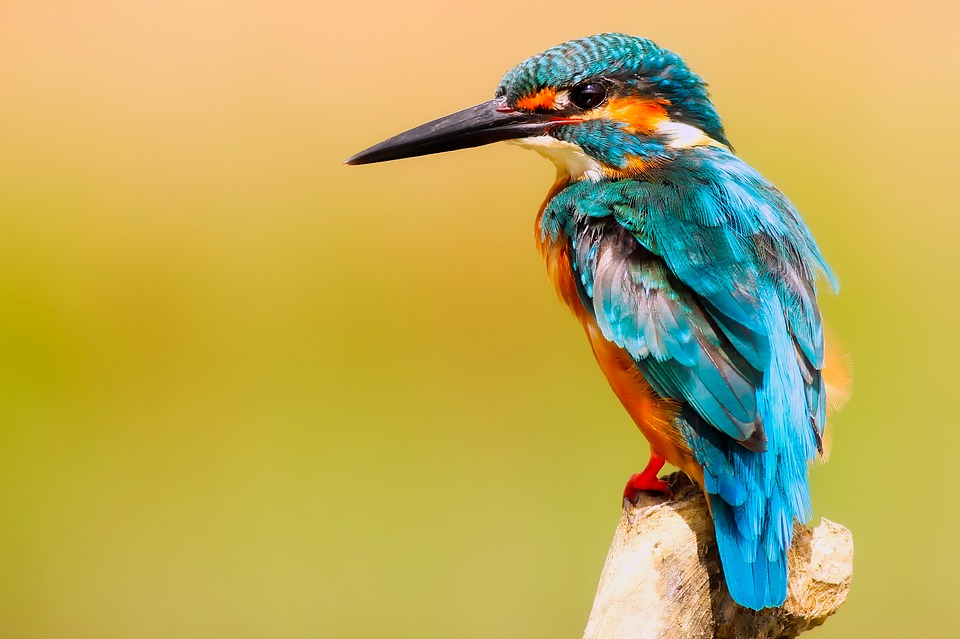
\includegraphics[width=.9\linewidth]{bird.jpg}
	\caption{A bird}
	\label{fig:bird}
\end{figure}
\end{texs*}
\end{minipage}
&
\begin{center}
	\captionsetup{type=figure}
	\vspace{5pt}
	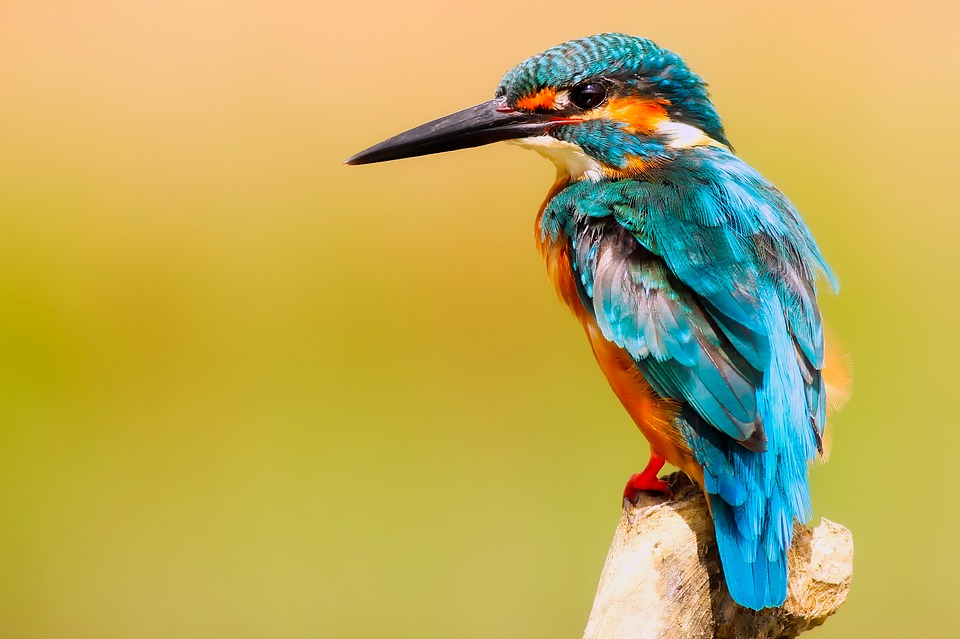
\includegraphics[width=\linewidth]{bird.jpg}
	\vspace{-10pt}
	\captionsetup{labelfont=normalfont, font=normalsize, width=\linewidth}
	\caption{A bird}
	\label{fig:bird2}
	\vspace{-10pt}
\end{center}
\\\bottomrule\end{tabular}

\begin{minipage}{\textwidth}
\subsection{Wrapping text}
\begin{wrapfigure}{r}{0.3\textwidth}
	\vspace{-25pt}
	\begin{center}
		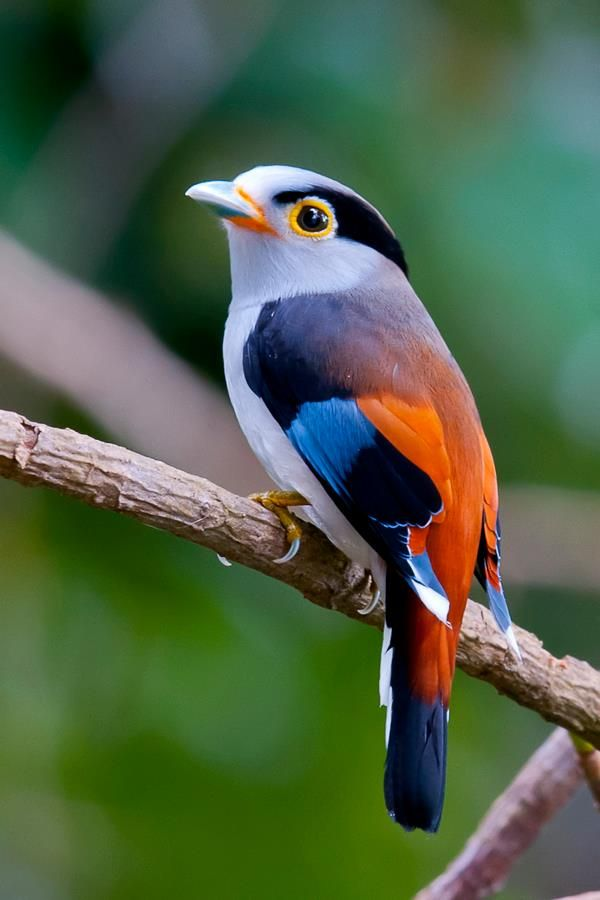
\includegraphics[width=.9\linewidth]{wrapbird.jpg}
	\end{center}
	\captionsetup{labelfont=normalfont, font=normalsize, width=\linewidth}
	\caption{A wrapped bird}
	\vspace{-80pt}
	\label{fig:wrapbird2}
\end{wrapfigure}

By default, figures in \LaTeX\ are placed between two lines of text, they take up the entire width of the page. However, sometimes it might be useful to have your text wrap around the figure on the side, especially when you have smaller tables or pictures. For this, use the package \gls{wrapfig}. To initiate a wrapped environment, use \tex!\begin{wrapfigure}[<lines>]{<pos>}{<width>}! where {\tt lines} is the number of lines you want the figure to span (optional), {\tt pos} is the position of the figure (either {\tt r} right or {\tt l} left) and {\tt width} is, of course, the width of the figure.

\vspace{10pt}
\begin{texlong*}{label=Example wrapped figure}
\begin{wrapfigure}{r}{0.3\textwidth}
	\begin{center}
		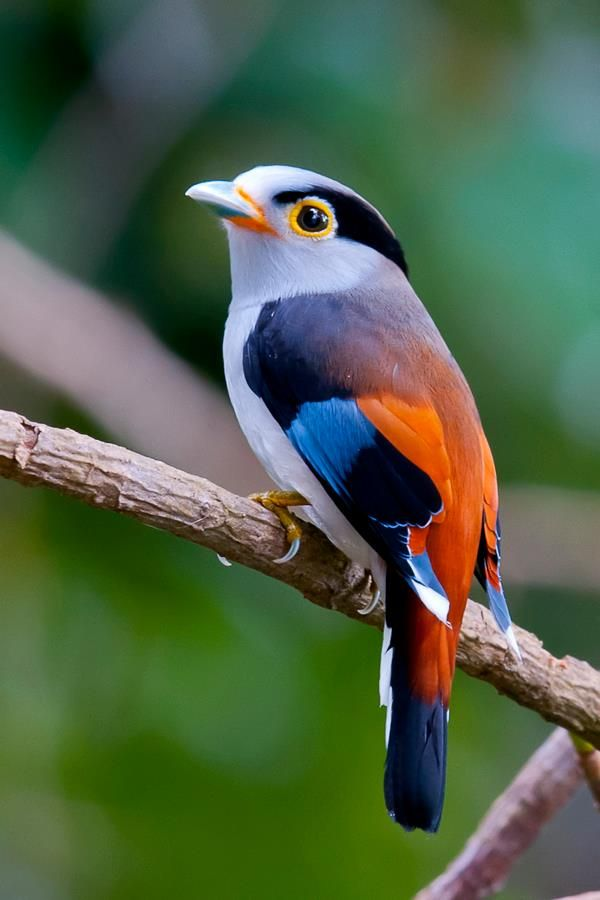
\includegraphics[width=.9\linewidth]{wrapbird.jpg}
	\end{center}
	\caption{A wrapped bird}
	\label{fig:wrapbird}
\end{wrapfigure}
\end{texlong*}
\vspace{10pt}

The placement of wrapped figures can be more difficult than normal figures. It can be the case that there is a lot of whitespace at the top or bottom of the wrapped figure, which causes text to look weird. This can be solved by inserting several \tex!\vspace{<length>}! commands in your figure with negative lengths. As for normal figures, a lot of trial-and-error is involved.
\end{minipage}

\subsection{Captions}
As you have already seen in the figures before, a figures and tables can be given a caption using \tex!\caption{<text>}!. This command will automatically recognize the current environment (e.g. figure and table), and will automatically but the correct text and number in place for you. Each different type of caption uses a separate counter.

By default, the caption system can be somewhat limiting. You might want to give captions to figures/images outside a {\tt figure} environment or style the appearance of your captions. This can be done using the \gls{caption} package, which provides the command \tex!\captionof{<type>}{<text>}! to insert a caption of the given {\tt type}. This can be for example {\tt table} and {\tt figure}.

The \gls{caption} package also enables you to customize the styling of your captions. This can be set in the options of the package, or using \tex!\captionsetup{<options>}!. The package provides many options, such as {\tt width}, {\tt font}, {\tt labelfont} and {\tt textfont}. The option {\tt position} is also interesting, since it specifies where the caption is with respect to the figure/table. This allows the package to correctly set the whitespace.

\vspace{5pt}
\begin{tabular}{p{.47\textwidth}m{.47\textwidth}}\toprule
\begin{minipage}{\linewidth}
\begin{texs}
\captionsetup{labelfont=bf, font=small, width=.8\linewidth}
\captionof{figure}{This is a smaller caption that is limited in width and automatically overflows}
You can see the difference when putting normal, long text next to it and comparing the width.
\end{texs}
\end{minipage}
&
\captionsetup{labelfont=bf, font=small, width=.8\linewidth, type=figure}
\caption{This is a smaller caption that is limited in width and automatically overflows}
You can see the difference when putting normal, long text next to it and comparing the width.
\\\bottomrule\end{tabular}

\subsection{Subfigures}\label{sec:subfigures}
Sometimes, it is desirable to have multiple items in one figure, such that you have figures 1a, 1b, etc. For this, the package \gls{subcaption} can be used. This package provides the {\tt subfigure} and {\tt subtable} environments that can be nested within an existing {\tt figure} and {\tt table}. Using \tex!\caption{<text>}! you can then give titles to them. As an example:

\vspace{5pt}
\begin{texlong*}{label=Subfigures example}
\begin{figure}[!h]
	\centering
	\begin{subfigure}[t]{0.3155\textwidth}
		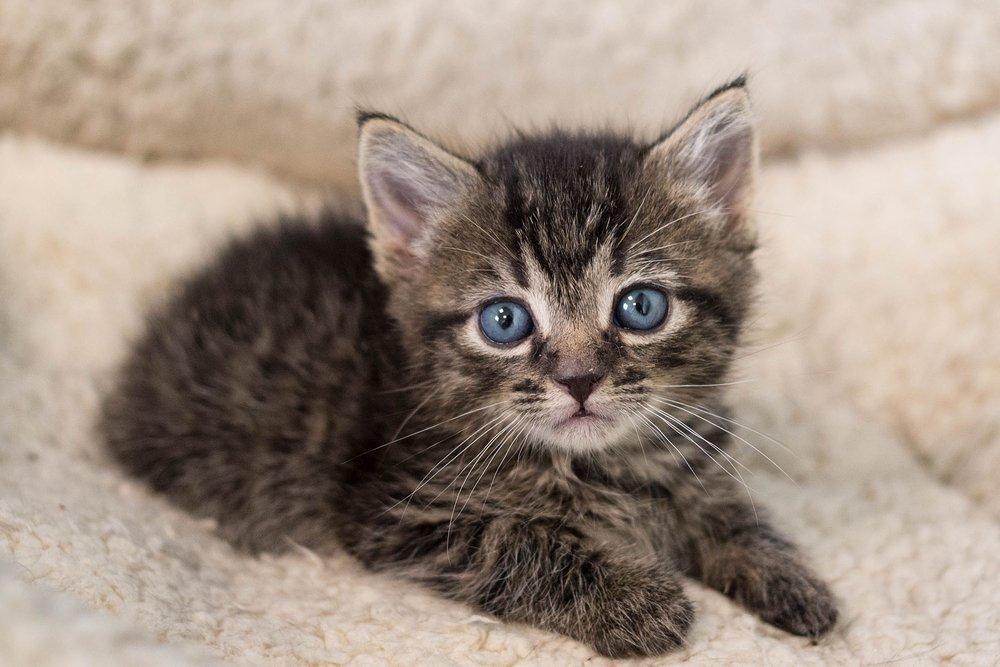
\includegraphics[width=\linewidth]{leftkitten.jpg}
		\caption{Left kitten}
	\end{subfigure}
	\begin{subfigure}[t]{0.3741\textwidth}
		
\includegraphics[width=\linewidth]{middlekitten.jpg}
		\caption{Middle kitten}
	\end{subfigure}
	\begin{subfigure}[t]{0.2104\textwidth}
		
\includegraphics[width=\linewidth]{rightkitten.jpg}
		\caption{Right kitten}
	\end{subfigure}
	\caption{Some kittens}
\end{figure}
\end{texlong*}
\vspace{-10pt}
\begin{figure}[!h]
	\centering
	\begin{subfigure}[t]{0.3155\textwidth}
		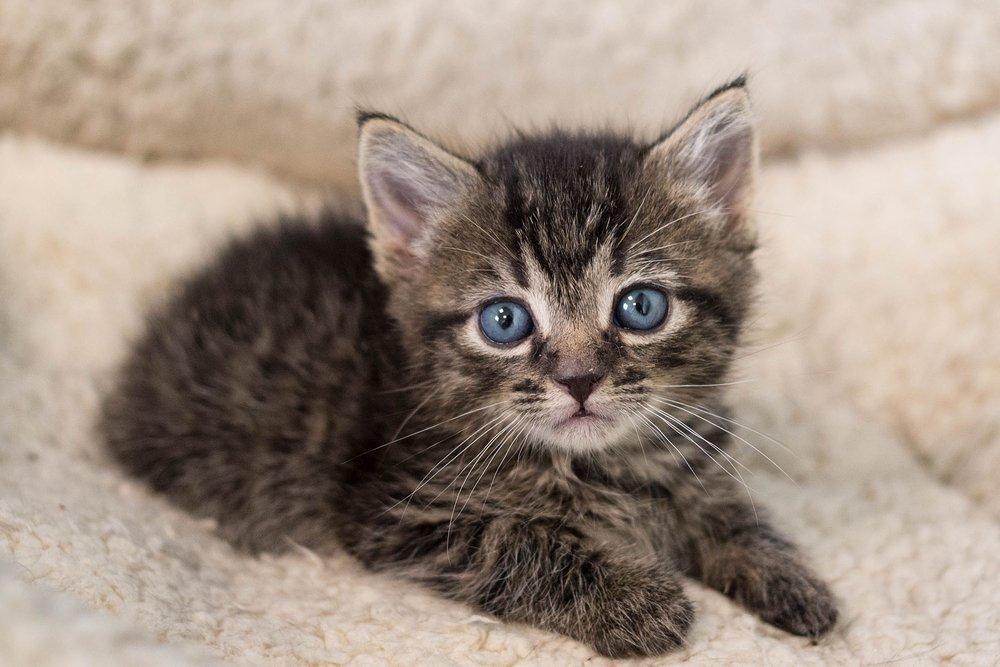
\includegraphics[width=\linewidth]{leftkitten.jpg}
		\caption{Left kitten}
	\end{subfigure}
	\begin{subfigure}[t]{0.3741\textwidth}
		
\includegraphics[width=\linewidth]{middlekitten.jpg}
		\caption{Middle kitten}
	\end{subfigure}
	\begin{subfigure}[t]{0.2104\textwidth}
		
\includegraphics[width=\linewidth]{rightkitten.jpg}
		\caption{Right kitten}
	\end{subfigure}
	\caption{Some kittens}
\end{figure}
\vspace{5pt}

You see that this works nicely, but the widths of the {\tt subfigure} are set to specific values as to make the pictures align. This is usually not a major problem, but in this case it would be nice if the pictures align properly. To do this automatically, there is some extra code necessary. I won't explain it, but the example is below.

\begin{figure}[!ht]
\begin{texlong*}{label=Subfigures with automatic sizing}
\begin{figure}[!h]
	\centering
	\newsavebox{\rowbox}
	\sbox\rowbox{\resizebox{.9\textwidth}{!}{
		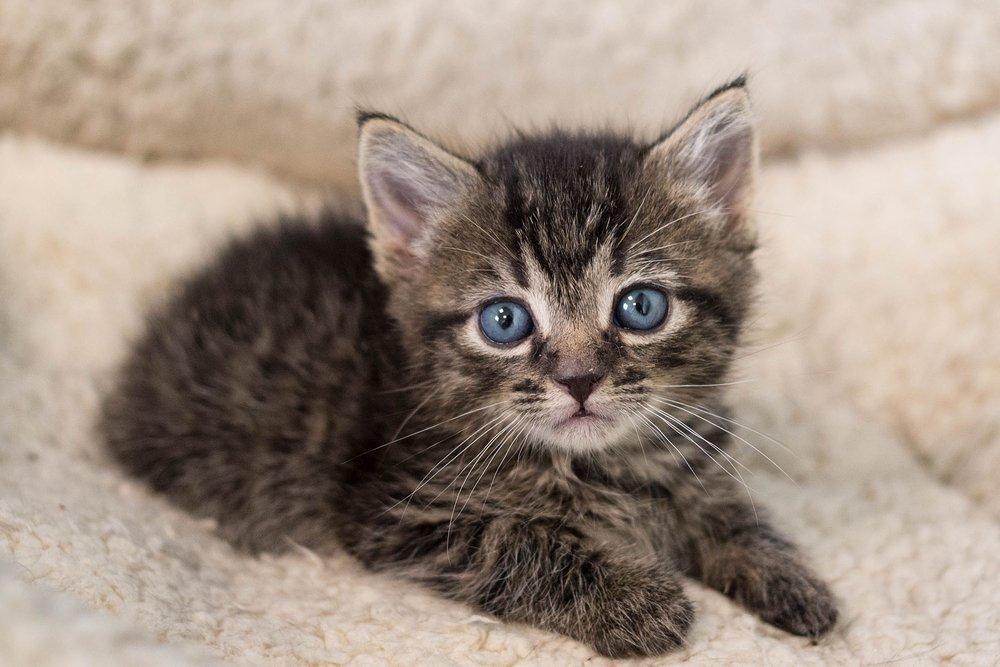
\includegraphics[height=10cm]{leftkitten.jpg}
		
\includegraphics[height=10cm]{middlekitten.jpg}
		
\includegraphics[height=10cm]{rightkitten.jpg}
	}}
	\newlength{\rowheight}
	\setlength{\rowheight}{\ht\rowbox}\hspace*{\fill}
	\subcaptionbox{Left kitten}{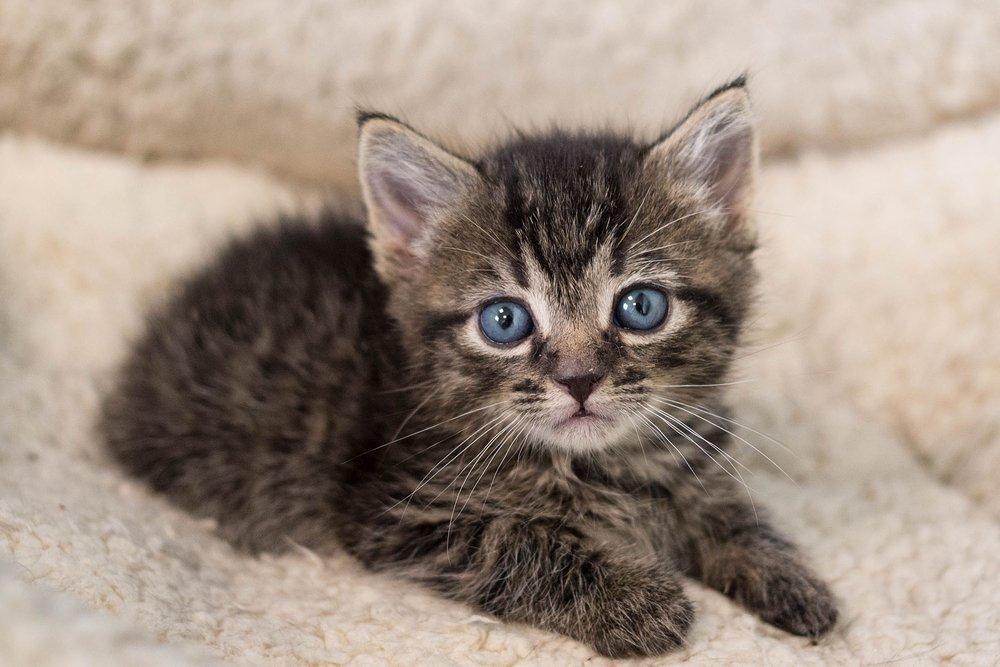
\includegraphics[height=\rowheight]{leftkitten.jpg}}\hfill
	\subcaptionbox{Middle kitten}{
\includegraphics[height=\rowheight]{middlekitten.jpg}}\hfill
	\subcaptionbox{Right kitten}{
\includegraphics[height=\rowheight]{rightkitten.jpg}}\hspace*{\fill}
	\caption{Some kittens}
\end{figure}
\end{texlong*}
	\vspace{10pt}
	\centering
	\newsavebox{\rowbox}
	\sbox\rowbox{\resizebox{.9\textwidth}{!}{
		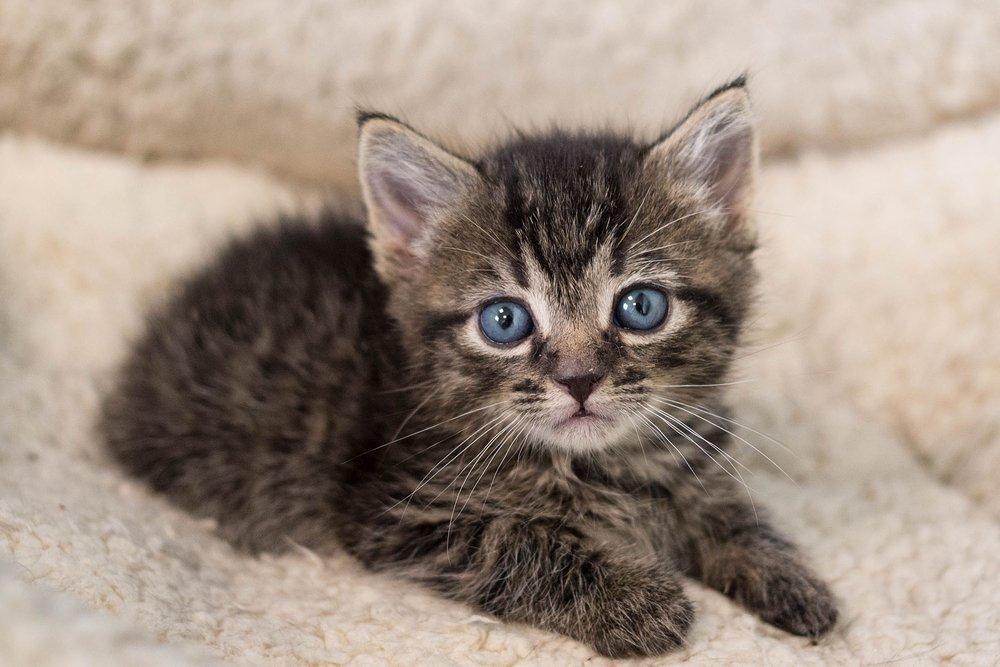
\includegraphics[height=10cm]{leftkitten.jpg}
		
\includegraphics[height=10cm]{middlekitten.jpg}
		
\includegraphics[height=10cm]{rightkitten.jpg}
	}}
	\newlength{\rowheight}
	\setlength{\rowheight}{\ht\rowbox}\hspace*{\fill}
	\subcaptionbox{Left kitten}{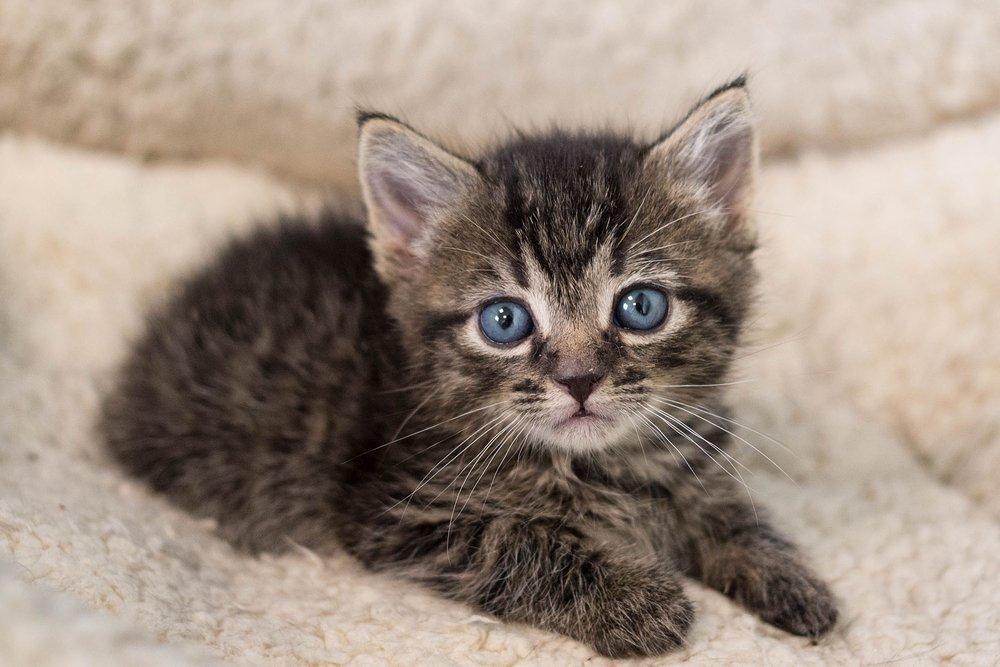
\includegraphics[height=\rowheight]{leftkitten.jpg}}\hfill
	\subcaptionbox{Middle kitten}{
\includegraphics[height=\rowheight]{middlekitten.jpg}}\hfill
	\subcaptionbox{Right kitten}{
\includegraphics[height=\rowheight]{rightkitten.jpg}}\hspace*{\fill}
	\caption{Some kittens}
\end{figure}

As an alternative to this, the \gls{floatrow} package can also be used. This package is more flexible and allows to do this with any content, not just figures from a file. For instructions on how to make this alignment work, see \underline{\href{http://ctan.triasinformatica.nl/macros/latex/contrib/floatrow/floatrow.pdf}{the documentation}}, paragraph 11.1.7.

\FloatBarrier
\subsection{Including pictures}
By default, it is not possible to include external pictures in your \LaTeX\ document. The package \gls{graphicx} enables this using the command \tex!\includegraphics[<options>]{<filename>}!. Here, in options you generally put the desired width or height of the picture, and in file you put the filename of the picture {\bf without spaces}. Spaces in filenames tend to break \LaTeX.

The file types supported differ for each compiler, but the most commonly used ones (PdfLaTeX, LuaLaTeX) support {\tt jpg}, {\tt png} and {\tt pdf}. The package \gls{epstopdf} also enable you to include {\tt eps} files. For example usage, see the figures above.

\subsection{Float barriers}
When including many figures in your document, they might get spread further and further down the document and might even `pollute' next chapters or sections. A built-in way to solve this is using \tex!\clearpage!, a command that puts all floats that do not yet have a position at this place, then goes on to the next page with the rest of the content. This way, several figures might end up at the pages before this command was called.

In some even more specific cases, it might not be desirable to insert a new page to clear all your floats. For example: that was the case with the last subfigure example, it kept drifting off into this section, something I did not want. I also did not want to include a page break here. The solution for this situation is provided by the package \gls{placeins} with \tex!\FloatBarrier! that enables you to place all `pending' floats at the current spot and then continue with the rest of the document directly.

%%%%%%%%%%%%%%%%%%%%%%%%%%%%%%%%%%%%%%%%%%%%%%%
%% Graphs %%%%%%%%%%%%%%%%%%%%%%%%%%%%%%%%%%%%%
%%%%%%%%%%%%%%%%%%%%%%%%%%%%%%%%%%%%%%%%%%%%%%%

\newpage
\section{Graphs}
In many scientific reports and articles, graphs are an integral part. There are multiple ways to make graphs and include them in your document. Often, graphs are generated using some external tool (Excel, Matlab, Mathematica), exported as JPG/PNG/PDF and then included as pictures in the document. This is a perfectly fine method, with one major disadvantage: they don't look in place. They generally don't share the \LaTeX\ fonts, its colors, etc. (The one exception to this is DataGraph (OSX only, paid) that generates stunning graphs that look just like native \LaTeX\ ones)

An alternative to using an external tool is to use some graphing library inside \LaTeX. The one I use the most is called \gls{pgfplots} which heavily relies on \gls{tikz} to make a range of graphs. In this chapter, I will be explaining the basics of this package. The possibilities are almost endless, as is clear from the enormous \underline{\href{http://pgfplots.sourceforge.net/gallery.html}{examples page}}. For more details on the options, refer to the \underline{\href{http://ctan.cs.uu.nl/graphics/pgf/contrib/pgfplots/doc/pgfplots.pdf}{566 page documentation}}.

\subsection{Basics}
All fun is happening inside the {\tt axis} environment, which lives inside a {\tt tikzpicture} environment. Therefore, the basic syntax is:

\vspace{5pt}
\begin{tabular}{p{.47\textwidth}>{\centering\arraybackslash}m{.48\textwidth} @{}}\toprule
\begin{minipage}{\linewidth}
\begin{texs}
\begin{tikzpicture}
	\begin{axis}[options]
		% Add plots
	\end{axis}
\end{tikzpicture}
\end{texs}
\end{minipage}
&
\begin{tikzpicture}
	\begin{axis}[height=5cm, width=7cm]
		% Add plots
	\end{axis}
\end{tikzpicture}
\\\bottomrule\end{tabular}
\vspace{5pt}

Here, {\tt options} is the place for many options of your graph. These options include things like {\tt title}, axis labels, grid settings and size.

\begin{tabular}{>{\tt}m{.2\textwidth}m{.74\textwidth}}\toprule
\bf Name & \bf Description \\\midrule
title & The title of the graph \\
xlabel & The title of the x-axis (also for {\tt y, z}). This is evaluated inside a maths environment, so use \tex!\text{...}! to get normal text \\
width & The width of the graph \\
height & The height of the graph \\
grid & Whether you want a grid on the background: {\tt major}, {\tt minor}, {\tt none}, {\tt both} \\
minor x tick num & (also for {\tt y, z}) Number of ticks in the minor grid per step in major grid \\
xmin, xmax & (also for {\tt y, z}) The range of x-values to plot \\
axis x line & (also for {\tt y, z}) Where the axis should show. Default both sides of the plot, options include {\tt left}, {\tt right}, {\tt top}, {\tt bottom}, {\tt middle} \\
xmode & (also for {\tt y}, {\tt z}) Whether the axis should be {\tt log}arithmic or {\tt linear} (default linear) \\
\bottomrule
\end{tabular}

\subsection{Function plots}
The easiest plots to do are function plots, so things like plotting $x^2$, $\sin(x)$ or even more complicated things like $\theta \to \left(\cos(\frac{3}{2}\theta)\cos\theta, \cos(\frac{3}{2}\theta)\sin\theta\right)$ and $z = (x+2)^2 + 4y^2$.

\vspace{10pt}
\captionsetup{type=figure}
\begin{scaletikz}
\begin{tikzpicture}
\begin{groupplot}[group style={group size=4 by 1},height=1/4*\textwidth,width=1/4*\textwidth]
\nextgroupplot[xmin=-2, xmax=2, ymin=0, ymax=4, axis y line=middle, axis x line=bottom]
\addplot[domain=-2:2, red] {x^2};
\nextgroupplot[xmin=0, xmax=2*pi, ymin=-1, ymax=1, axis x line=middle, axis y line=left]
\addplot[domain=0:2*pi, blue, samples=50] {sin(deg(x))};
\nextgroupplot[axis y line=middle, axis x line=middle, xmin=-.1, xmax=1, ymin=-1, ymax=.4]
\addplot[domain=0:4*pi, samples=1000] ({cos(1.5*deg(x))*cos(deg(x))},{cos(1.5*deg(x))*sin(deg(x))});
\nextgroupplot[colormap/cool, xmin=-4, xmax=0, ymin=-1, ymax=1, zmin=0, zmax=8, z post scale=.7, view={20}{40}, 3d box=complete]
\addplot3[surf, samples=100, domain=-4:0, y domain=-1:1] {4*y^2+(x+2)^2};
\end{groupplot}
\end{tikzpicture}
\end{scaletikz}
\begin{centering}
\caption{Some example plots that are possible with \gls{pgfplots}}
\end{centering}
\vspace{10pt}

As you can already see, it is possible to plot both 2D- and 3D-functions. Also, both explicit ($y = f(x)$) and parametrized functions ($t \to (x(t), y(t))$) are supported. Unfortunately, implicit functions like the unit circle ($x^2 + y^2 = 1$) are not supported and need to be either parametrized or plotted in multiple parts (one part of each $x_\pm = \pm \sqrt{1-y^2}$ in this case). However, within those conditions, the library is quite flexible and can plot almost anything.

\subsubsection{2D plots}
To plot a 2D-function, we use the command \tex!\addplot [<options>] {<function>};! (note the semicolon!). In the options it is possible to define the color of the line, define some domain to be plotted or (useful for parametrized functions) set how many samples should be taken within your plotted domain. Within the curly brackets {\tt \{\}} the function should be specified in terms of {\tt x}. This gives the following code for our $y=x^2+x-4$.

\begin{tabular}{p{.47\textwidth}>{\centering\arraybackslash}m{.48\textwidth} @{}}\toprule
\begin{minipage}{\linewidth}
\begin{texs}
\begin{tikzpicture}
	\begin{axis}[axis y line=middle, axis x line=middle]
		\addplot[domain=-2:2, red] {x^2+x-4};
	\end{axis}
\end{tikzpicture}
\end{texs}
\end{minipage}
&
\begin{tikzpicture}
	\begin{axis}[axis y line=middle, axis x line=middle, height=5cm, width=7cm]
		\addplot[domain=-2:2, red] {x^2+x-4};
	\end{axis}
\end{tikzpicture}
\\\bottomrule\end{tabular}
\vspace{5pt}

For parametrized functions, replace the function inside the curly brackets with two sets of them wrapped inside normal brackets as follows: {\tt (\{a(x)\},\{b(x)\})}. The first function describes {\tt x}, the other {\tt y}. Both functions should be defined in terms of {\tt x} (confusing, I know). It is recommended to define the number of samples that should be taken, to avoid sharp edges. As an example, for the famous Lissajous curve:

\begin{tabular}{p{.47\textwidth}>{\centering\arraybackslash}m{.48\textwidth} @{}}\toprule
\begin{minipage}{\linewidth}
\begin{texs}
\begin{axis}
	\addplot[domain=0:2*pi, blue, samples=400]
		({cos(3*deg(x))}, {sin(2*deg(x))});
\end{axis}
\end{texs}
\end{minipage}
&
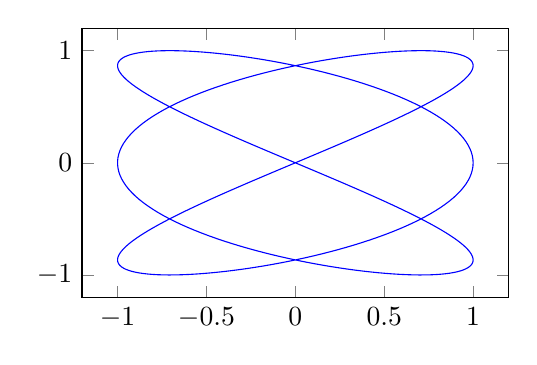
\begin{tikzpicture}
	\begin{axis}[width=7cm, height=5cm]
		\addplot[domain=0:2*pi, blue, samples=400] ({cos(3 * deg(x))}, {sin(2 * deg(x))});
	\end{axis}
\end{tikzpicture}
\\\bottomrule\end{tabular}
\vspace{5pt}

Note that all trigonometric functions in \gls{pgfplots} are based on degrees and not radians, so in order to use them with radians, the input should be converted to degrees using {\tt deg(x)}, as done in the example above.

It is also possible to work with a polar coordinate system, which might be more useful for some functions. For this, the pgfplots library {\tt polar} should be included and all code should be in the {\tt polaraxis} environment. Besides that, the function specified in \tex!\addplot;! should give the radius ($r(\theta)$) instead of $y$. For a more advanced example, with a butterfly curve, we get:

\vspace{5pt}
\begin{tabular}{p{.47\textwidth}>{\centering\arraybackslash}m{.47\textwidth}}\toprule
\begin{minipage}{\linewidth}
\begin{texs*}{fontsize = \fontsize{8pt}{10.5pt}}
% In your preamble
\usepackage{pgfplots}
\usepgfplotslibrary{polar}

% ...
% In your document somewhere
\begin{tikzpicture}
	\begin{polaraxis}
		\addplot[red, domain=0:7200, samples=5000] {...};
	\end{polaraxis}
\end{tikzpicture}
\end{texs*}
\end{minipage}
&
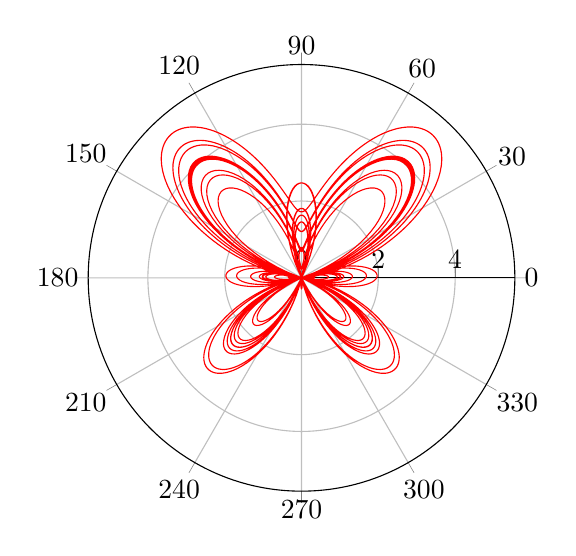
\begin{tikzpicture}
	\begin{polaraxis}[width=7cm, height=7cm]
		\addplot[red, domain=0:7200, samples=5000] {e^(sin(x)) - 2*cos(4*x) + (sin((2*x-180)/24))^5};
	\end{polaraxis}
\end{tikzpicture}
\\\bottomrule\end{tabular}

\subsubsection{3D plots}
It is also possible to generate 3D plots in \gls{pgfplots}. However, this will get you into trouble for more complex graphs. Plotting more than 1 function will get you into trouble, and also more advanced functions might give problems with the memory limit or something else. For the simpler functions \gls{pgfplots} is fine, but for more complex ones, it might be best to use an external tool.

The syntax of 3D plots is quite similar to 2D plots, except that the function to call is now called \tex!\addplot3 [<options>] {<function>};! where the 3 indicates that this is a 3D function. The options are again quite similar, with now an added {\tt y domain} for the second variable. The function to be specified between the {\tt \{\}} is now a function of $z = f(x, y)$, or again parametrized with $t \to (x(t), y(t), z(t))$ (so you have to specify 3 variables!).

The {\tt axis} environment also has some extra options that are useful for 3D plots. With {\tt view=\{a\}\{b\}} it is possible to define the angle from which you view the graph and with {\tt 3d box=complete} it is possible to get lines on all edges of the `box' that is plotted. In the {\tt addplot3} command, options have been added for the domain of {\tt y} ({\tt y domain}) and the number of samples of {\tt y} ({\tt samples y}). For 3D surfaces there are multiple plot types, {\tt mesh} is for contours only (like a net), {\tt surf} is to fill the surface completely (and show contour lines).

It is also possible to color your surface, to make it clearer what its $z$-value is. This can be done using color maps, that have to be set in the options of your plot command. The syntax for this is {\tt [colormap/name, <options>]} where name is the name of the color map you want to use. Some of the predefined color maps are: {\tt hot}, {\tt jet}, {\tt blackwhite}, {\tt cool} and {\tt bluered}.

As an example, below the parametrized function $(t, u) \to \big(2 + 2\tanh[2](\textstyle\frac{1}{2}t)\cdot\cos(u);\ 2 + 2\tanh[2](\textstyle\frac{1}{2}t)\cdot\sin(u);\ t)$ is plotted, with a color map and 40 samples in both variables. Note that the option {\tt z buffer=sort} is defined, this is to make sure that the elements in the back don't overlap the elements in the front.

\begin{tabular}{p{.47\textwidth}>{\centering\arraybackslash}m{.47\textwidth}}\toprule
\begin{minipage}{\linewidth}
\begin{texs*}{fontsize = \fontsize{8pt}{10.5pt}}
\begin{axis}[colormap/cool, view={30}{20}]
	\addplot3[surf, z buffer=sort, samples=40, samples y=40, domain=-3:3, y domain=0:2*pi]
		(
			{(2 + 2 * tanh(.5*x)^2) 
				* cos(deg(y))},
			{(2 + 2 * tanh(.5*x)^2)
				* sin(deg(y))}, 
			{x}
		);
\end{axis}
\end{texs*}
\end{minipage}
&
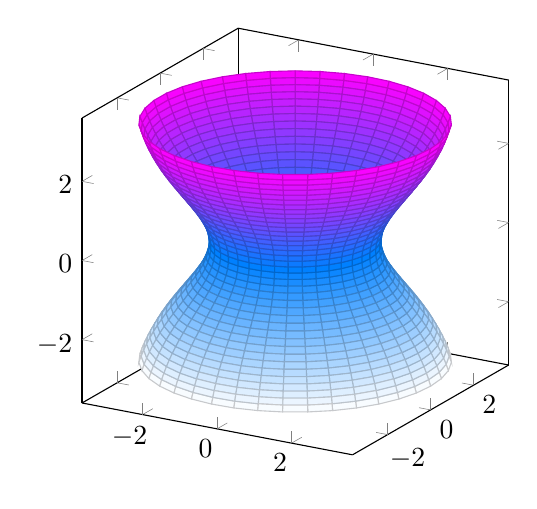
\begin{tikzpicture}
\begin{axis}[colormap/cool,width=7cm,height=7cm,view={30}{20}]
\addplot3[surf, z buffer=sort, samples=40, samples y=40, domain=-3:3, y domain=0:2*pi]
	({(2 + 2 * tanh(.5*x)^2) * cos(deg(y))}, {(2 + 2 * tanh(.5*x)^2) * sin(deg(y))}, x);
\end{axis}
\end{tikzpicture}
\\\bottomrule\end{tabular}

\subsection{Data plots}\label{sec:pgf_dataplots}
A very important and often-used plot is of course a plot of measurement data. Various types of plots are available, such as scatter plots, bar plots, stacked plots, filled plots (area under the line is colored), boxplots and many more. In this document, only scatter plots will be discussed. For the other types of plots, refer to the documentation of \gls{pgfplots}. All other types of plots are very similar to scatter plots and require only one or two options to be set.

In this part we will focus on getting your measurement data in your graph. There are two main ways of plotting your data points. The first is by defining them all in the {\tt tikzpicture} code as coordinates. The other is by using a separate data file. The latter is the easiest if you export your data from another program such as Matlab or Mathematica, and the only option if you want to fit a function through the data later on.

\subsubsection{Simple coordinates}
\begin{sloppypar}
To plot simple coordinates you can use \tex!\addplot [<options>] coordinates {<coords>};! where again {\tt options} is for your options and in this case you put a list of coordinates inside the curly brackets {\tt coords}. It is also possible to specify error bars for your data points, see the example below. More information on error bars can be found in section \ref{sec:pgf_error}. A useful option for these plots is {\tt only marks} that hides the line that (by default) connects the data points. A basic example showcasing the possibilities:
\end{sloppypar}

\vspace{5pt}
\begin{tabular}{p{.47\textwidth}>{\centering\arraybackslash}m{.47\textwidth}}\toprule
\begin{minipage}{\linewidth}
\begin{texs}
\begin{axis}[minor y tick num=1]
	\addplot[red, only marks,
			error bars/.cd, 
			x dir=both, x explicit, 
			y dir=both, y explicit
		] coordinates {
			(1,1) +- (0.1, 0.3)
			(2,1.8) +- (0.4, 0.2)
			(3.2,3.8) += (0.2, 0.8) -= (0.5, 0.2)
			(4.8,5.2) +- (1, 0.3)
		};
\end{axis}
\end{texs}
\end{minipage}
&
\begin{tikzpicture}
\begin{axis}[width=7cm,height=6cm, minor y tick num = 1]
\addplot[red, only marks, error bars/.cd, x dir=both, x explicit, y dir=both, y explicit] coordinates {
	(1,1) +- (0.1, 0.3)
	(2,1.8) +- (0.4, 0.2)
	(3.2,3.8) += (0.2, 0.8) -= (0.5, 0.2)
	(4.8,5.2) +- (1, 0.3)
};
\end{axis}
\end{tikzpicture}
\\\bottomrule\end{tabular}

\subsubsection{External source}\label{sec:pgf_dataplots_external}
The basic coordinates method demonstrated above is easy to start with, but with larger data sets it becomes cumbersome to have all data in your latex code all the time. Also it might require a lot of manual labour to convert all your data to the correct format, especially if the data is extracted from another program such as Matlab or Mathematica. The solution for this is to save your data in any external file, which should be formatted as simple text with columns separated by white space (at least one tab or space) and rows separated by newlines. Other options are possible using the \gls{pgfplotstable}.

\comment{Note on including your data in your \LaTeX\ file}{
Sometimes it might be inconvenient to use separate files for your measurement data and if you're like me you'd like to keep all the data in one file. Even when using external files as a data source for your graphs, it is still possible to define your data inside latex. Simply include the package \gls{filecontents} and put your data inside the {\tt filecontents} environment using \tex!\begin{filecontents}{<filename>} data \end{filecontents}!. The contents of the environment will then be stored in the file with your filename.}

\begin{sloppypar}
To use an external file as data source for your graph, put {\tt table} in your \tex!\addplot;! command: \tex!\addplot [<options>] table [<data specification>] {<filename>};!. Inside, there is the usual {\tt options} part for the usual options. New is the {\tt data specification}, here you define what column is the data for what axis. The {\tt filename} is quite straightforward, but keep in mind that {\bf file names in \LaTeX\ cannot have spaces in them}! This might work in some places but usually yields very unpredictable behaviour.
\end{sloppypar}

In this case, an example is again the easiest way to show how this works:

\begin{filecontents}{_graph-data/table_example.dat}
X	Y	X_err	Y_err
1	1	0.1		0.3
2	1.8	0.4		0.2
3.2	3.8	0.2		0.8
4.8	5.2	1		0.3
\end{filecontents}
\begin{tabular}{p{.47\textwidth}>{\centering\arraybackslash}m{.47\textwidth}}\toprule
\begin{minipage}{\linewidth}
\begin{texs*}{fontsize = \fontsize{8pt}{10.5pt}}
% Data format:
% X   Y   X_err   Y_err
% 1   1   0.1     0.3
% ...

\begin{axis}[
		minor y tick num=3,
		minor x tick num=3,
		grid=both
	]
	\addplot[red, only marks, 
			error bars/.cd, 
			x dir=both, x explicit, 
			y dir=both, y explicit
		] table [
			x=X, y=Y, 
			x error=X_err, y error=Y_err
		] {<filename>};
\end{axis}
\end{texs*}
\end{minipage}
&
\begin{tikzpicture}
\begin{axis}[width=7cm,height=6cm, minor y tick num=3, minor x tick num=3, grid=both]
\addplot[red, only marks, error bars/.cd, x dir=both, x explicit, y dir=both, y explicit] table [x=X, y=Y, x error=X_err, y error=Y_err] {_graph-data/table_example.dat};
\end{axis}
\end{tikzpicture}
\\\bottomrule\end{tabular}

\subsection{Error bars}\label{sec:pgf_error}
Another useful and important feature in \gls{pgfplots} is the ability to show error bars. The error bars are quite flexible, it is possible to define absolute and relative values, but also expressions/functions such as $\sqrt{x}$. Furthermore, it is possible to define separate error values for both the positive and negative directions (so-called asymmetric errors). To enable error bars on any (data) plot, include the option {\tt error bars/.cd} in the {\tt addplot} command. Include this as the last option, all other options you define after this will be about the errors.

First, you have to define what directions you want your error bars to appear in. For this, use {\tt x dir} (or {\tt y} or {\tt z}) and specify what type of bars you want. The options are {\tt none} (no error bars), {\tt plus} (only in the positive direction), {\tt minus} (only in the negative direction) and {\tt both} (error bars in both directions). The actual value has to be specified separately. In case of {\tt both} it is also possible to specify different values for the positive and negative direction.

The easiest way to add error bars to your measurements is to include them in your data set, as done in section \ref{sec:pgf_dataplots}. Then in your options, define that the error is given explicitly, by adding {\tt x explicit} (or {\tt y}, {\tt z}). It is also possible to make the error constant for all your measurement values, then add the options {\tt x fixed = value} where you replace {\tt value} by the error value. For both cases there is also the alternative {\tt x explicit relative} (and {\tt x fixed relative}) that states that the given value is a relative error (a factor, 1 = 100\%).

For the {\tt table} plot type it is also possible to specify separate positive and negative errors, put this information in separate columns and include them in the options using {\tt x error plus} and {\tt x error minus} and omit the default {\tt x error}. More advanced is the ability to make each of these possible errors a mathematical expression rather than a value. This is done using {\tt x error expr} (similar for other axes). The expression given can make use of the data of other columns in the same row using \tex!\thisrow{<column>}!.

The example below showcases all functionality. The absolute error in positive $x$ direction is given in the data file, the absolute error in negative x direction is given by the expression $\bar{x} = \sin[2](100x)$ (remember that sin works in degrees), the relative error in both directions for y is 30\%.

\begin{filecontents}{_graph-data/error_example.dat}
X	Y	X_err+
1	1	.2
2	1.8	.4
3.2	3.8	.2
4.8	5.2	1
\end{filecontents}
\begin{tabular}{p{.48\textwidth}>{\centering\arraybackslash}m{.47\textwidth} @{}}\toprule
\begin{minipage}{\linewidth}
\begin{texs*}{fontsize=\fontsize{8pt}{10.5pt}}
\begin{axis}
	\addplot[red, only marks, 
			error bars=./cd, 
			x dir=both, x explicit, 
			y dir=both, y fixed relative=.3
		] table [
			x=X, y=Y, 
			x error plus=X_err+, 
			x error minus expr={sin(\thisrow{X}*100)^2}
		] {<filename>};
\end{axis}
\end{texs*}
\end{minipage}
&
\begin{tikzpicture}
\begin{axis}[width=8cm, height=6cm]
\addplot[red, only marks, error bars=./cd, x dir=both, x explicit, y dir=both, y fixed relative=.3] table [x=X, y=Y, x error plus=X_err+, x error minus expr={sin(\thisrow{X}*100)^2}] {_graph-data/error_example.dat};
\end{axis}
\end{tikzpicture}
\\\bottomrule\end{tabular}

\subsection{Fitting a function}
When you have plotted your data, the next logical thing to do is to fit some function through your data. Often, you'll have some simple linear relationship $y = ax + b$ where you want to determine your $a$ and $b$. In other cases you might want to fit more complex functions such as $y = a\sin(bx + c)$ through your data. Luckily, both are possible, but unfortunately not with \gls{pgfplots} only. To properly fit a function, we need the help of the external tool {\tt gnuplot}.

\subsubsection{Setting up {\tt gnuplot}}\label{sec:pgf_gnuplot}
When working online in either Overleaf or ShareLatex, everything is already set up correctly and you can start working with {\tt gnuplot} directly, so you can skip this part. When working offline, first install {\tt gnuplot} from the \underline{\href{http://www.gnuplot.info/download.html}{download site}}. Make sure to add {\tt gnuplot} to your {\tt PATH} (option in the setup). After that, your \LaTeX\ program needs to be set up correctly: the parameter {\tt --shell-escape} needs to be added to the compile command. For some programs I added instructions below, for your specific program please search online.

\paragraph{TeXstudio}
To modify the compile command, go to Options -> Configure TeXstudio -> Commands. Then add {\tt -shell-escape} just after the part with {\tt -synctex=1} in the top 4 entries (LaTeX, PdfLaTeX, XeLaTeX and LuaLaTeX).

\paragraph{TeXpad}
TeXpad has functionality built-in that automatically enables this option. If, for some reason, this doesn't work, you can manually enable it by switching the option `Shell Escape' in the typeset configuration (click on the arrow next to `Typeset' in the toolbar, choose `Manual' instead of `Auto-sense').

\subsubsection{Calling {\tt gnuplot}}
{\tt gnuplot} is a powerful plotting tool that can plot many different types of graphs. The program is script-based, so you need to put in a script to get out your graphs. It can be called using the command \tex!\addplot [raw gnuplot, <options>] gnuplot {<code>};! where again, {\tt options} are the usual options for the plot and {\tt code} is the code to be executed. I will not discuss the full functionality of {\tt gnuplot} here, since that is beyond the scope of this document. For more information, refer to the documentation. As a quick example:

\begin{tabular}{p{.47\textwidth}>{\centering\arraybackslash}m{.47\textwidth}}\toprule
\begin{minipage}{\linewidth}
\begin{texs}
\begin{axis}
\addplot[raw gnuplot, red] gnuplot {
	f(x) = a*x^2;
	a = 2;
	plot [x=-2:2] f(x);
};
\end{axis}
\end{texs}
\end{minipage}
&
\begin{tikzpicture}
\begin{axis}[width=7cm,height=5cm]
\addplot[raw gnuplot, red] gnuplot {
	f(x) = a*x^2;
	a = 2;
	plot [x=-2:2] f(x);
};
\end{axis}
\end{tikzpicture}
\\\bottomrule\end{tabular}

\subsubsection{Making a fit}
To do a fit through some test data, it is easiest to have your data in an external file, as outlined in section \ref{sec:pgf_dataplots_external}. Below, I will provide an example with the basic script to do a linear fit on some data. It is easy to adapt this to your situation, by changing {\tt f(x)}, adding more variables, or changing the indexes of your columns.

\begin{tabular}{p{.57\textwidth}>{\centering\arraybackslash}m{.37\textwidth}}\toprule
\begin{minipage}{\linewidth}
\begin{texs*}{fontsize=\fontsize{8pt}{10.5pt}}
\addplot[red, only marks, mark=x] table [x=X, y=Y] {<filename>};
\addplot[raw gnuplot, red] gnuplot {
\end{texs*}
\vspace{-34pt}
\begin{gnuplots*}{fontsize=\fontsize{8pt}{10.5pt}}
	# Function to fit
	f(x) = a*x + b;
	# Initial guesses for all variables
	a = 1; b = 1;
	# Fit command.
	fit f(x) '<filename>' using 1:2 via a,b;
	# Plot the function for the given domain
	plot [x=0:6] f(x);
\end{gnuplots*}
\vspace{-34pt}
\begin{texs*}{fontsize=\fontsize{8pt}{10.5pt}}
};
\end{texs*}
\end{minipage}
&
\begin{tikzpicture}
\begin{axis}[xmin=0, xmax=6, ymin=0, ymax=6, width=6cm, height=5cm]
\addplot[red, only marks, mark=x] table [x=X, y=Y] {_graph-data/table_example.dat};
\addplot[raw gnuplot, red] gnuplot {
	f(x) = a*x + b;
	a = 1; b = 1;
	fit f(x) '_graph-data/table_example.dat' using 1:2 via a,b;
	plot [x=0:6] f(x);
};
\end{axis}
\end{tikzpicture}
\\\bottomrule\end{tabular}

The {\tt fit} command is used to calculate the best fit for the variables through the data and has the following syntax: \gnup!fit <function> <filename> using <x>:<y> via <vars>;! where {\tt function} is the function to fit, {\tt filename} is the file with the data, {\tt x} and {\tt y} are the indices of the columns for X and Y (starting at 1) and {\tt vars} are the variables in the function that have to be fitted. A more complex example, based on a real experiment I did some time ago:

\begin{filecontents}{_graph-data/visibility_curves.dat}
X,Y
0,6853.5
10,6151.5
20,5167
30,4149.5
40,2845
50,1737
60,870.5
70,345
80,189
90,441.5
100,1094.5
110,2077
120,3281
130,4485.5
140,5652
150,6699.5
160,7222
170,7481
180,7353.5
190,6706.5
200,5587
210,4464
220,3152.5
230,1956.5
240,967
250,366
260,192
270,474
280,1200.5
290,2133.5
300,3404.5
310,4639
320,5745
330,6501
340,6994.5
350,7126.5
\end{filecontents}
\begin{tabular}{p{.51\textwidth}>{\centering\arraybackslash}m{.44\textwidth} @{}}\toprule
\begin{minipage}{\linewidth}
\begin{texs*}{fontsize=\fontsize{8pt}{10.5pt}}
\addplot[red, mark=x, only marks] table [x=X, y=Y] {<filename>};
\addplot[raw gnuplot, red, mark=none] gnuplot {
\end{texs*}
\vspace{-34pt}
\begin{gnuplots*}{fontsize=\fontsize{8pt}{10.5pt},mathescape}
	f(x) = a*sin(b*x + c) + d;
	a = 3000; b=-2; c=100; d=4000;
	# Marks that $\sin$ should work with degrees
	set angles degrees;
	fit f(x) '<filename>' using 1:2 via a,b,c,d;
	plot [x=0:360] f(x);
\end{gnuplots*}
\vspace{-34pt}
\begin{texs*}{fontsize=\fontsize{8pt}{10.5pt}}
};
\end{texs*}
\end{minipage}
&
\begin{tikzpicture}
\begin{axis}[xmin=0, xmax=360, ymin=0, ymax=8000, width=7cm, height=6cm, minor x tick num=5]
\addplot[red, mark=x, only marks] table [x=X, y=Y, col sep=comma] {_graph-data/visibility_curves.dat};
\addplot[raw gnuplot, red, mark=none] gnuplot {
	f(x) = a*sin(b*x + c) + d;
	a = 3000; b=-2; c=100; d=4000;
	set angles degrees;
	set datafile separator ',';
	fit f(x) '_graph-data/visibility_curves.dat' using 1:2 via a,b,c,d;
	plot [x=0:360] f(x);
};
\end{axis}
\end{tikzpicture}
\\\bottomrule\end{tabular}

\subsubsection{Incorporating error bars}
It is also possible to fit data sets while incorporating errors in the measurement data. These errors should be stored in separate columns in your data file. The commands for incorporating errors are:\newline
\gnup!fit <function> <filename> using <x>:<y>:<xerror> xerror via a,b;! \newline
\gnup!fit <function> <filename> using <x>:<y>:<yerror> yerror via a,b;! \newline
\gnup!fit <function> <filename> using <x>:<y>:<xerror>:<yerror> xyerrors via a,b;! \newline
for errors in $x$-direction only, errors in $y$-direction only and errors in both directions, respectively. Here {\tt <xerror>} and {\tt <yerror>} are the column indices of the columns where the error value is stored.

Each of the column index markers can be replaced with an expression as well. Put this expression in between normal brackets {\tt ()}. Within such an expression it is possible to refer to the other columns using {\tt \$<i>} where {\tt i} is the index of the other column. As an example:

\begin{filecontents}{_graph-data/error_fit_example.dat}
X	Y	Y_err
1	1	.2
2	1.8	.4
3.2	3.8	.2
4.8	5.2	1
\end{filecontents}
\begin{tabular}{p{.52\textwidth}>{\centering\arraybackslash}m{.42\textwidth}}\toprule
\begin{minipage}{\linewidth}
\begin{texs*}{fontsize=\fontsize{8pt}{10.5pt}}
\addplot[
	red, only marks, error bars=./cd,
	x dir=both, x explicit,
	y dir=both, y explicit
] table [
	x=X, y=Y,
	x error expr={sin(\thisrow{X}*100)^2},
	y error=Y_err
] {<filename>};
\addplot[raw gnuplot, red, mark=none] gnuplot {
\end{texs*}
\vspace{-34pt}
\begin{gnuplots*}{fontsize=\fontsize{8pt}{10.5pt}}
	f(x) = a*x + b;
	a = 1; b = 1;
	set angles degrees;
	fit f(x) '<filename>' using 1:2:(sin($1*100)^2):3 xyerrors via a,b;
	plot [x=0:6] f(x);
\end{gnuplots*}
\vspace{-34pt}
\begin{texs*}{fontsize=\fontsize{8pt}{10.5pt}}
};
\end{texs*}
\end{minipage}
&
\begin{tikzpicture}
\begin{axis}[xmin=0, xmax=6, ymin=0, ymax=6, width=6cm, height=5cm]
\addplot[red, only marks, error bars=./cd, x dir=both, x explicit, y dir=both, y explicit] table [x=X, y=Y, x error expr={sin(\thisrow{X}*100)^2}, y error=Y_err] {_graph-data/error_fit_example.dat};
\addplot[raw gnuplot, red, mark=none] gnuplot {
	f(x) = a*x + b;
	a = 1; b = 1;
	set angles degrees;
	fit f(x) '_graph-data/error_fit_example.dat' using 1:2:(sin($1*100)^2):3 xyerrors via a,b;
	set datafile commentschars '$';
	plot [x=0:6] f(x);
};
\end{axis}
\end{tikzpicture}
\\\bottomrule\end{tabular}

\subsection{Legend entries}\label{sec:pgf_legend}
\begin{sloppypar}
Another important aspect of a graph is its legend, especially if multiple lines or data sets are plotted. Luckily, generating the legend is relatively easy. Simply put the command \tex!\addlegendentry{<name>}! (without semicolon!) after the \tex!\addplot;!. Note that this will add all plots in order, so if you do two \tex!\addplot;!'s and after that an \tex!\addlegendentry!, the entry added will be for the first plot. In order to skip a plot, add the option {\tt forget plot} to the \tex!\addplot;! command.
\end{sloppypar}

To determine the legend position, use the {\tt legend pos} option for the {\tt axis} environment. Possible values are each diagonal wind direction ({\tt north east}, {\tt south west}, etc) that will place the legend in one of these corners of the graph. Only {\tt north east} can also be combined with {\tt outer} (i.e. {\tt outer north east}), to place the legend outside the graph, next to it.

It is also possible to label your plots using \tex!\label{<name>}! and refer to them using \tex!\ref{<name>}!, the reference will then be the line style of the plot you refer to. Note that this does not work when using the {\tt external} library, as explained in \ref{sec:pgf_externalize}, you'll find a workaround there as well. As an example to combine all options:

\begin{tabular}{p{.47\textwidth}>{\centering\arraybackslash}m{.47\textwidth}}\toprule
\begin{minipage}{\linewidth}
\begin{texs*}{fontsize=\fontsize{8pt}{10.5pt}}
\begin{tikzpicture}
\begin{axis}[legend pos=outer north east]
	\addplot [red, domain=0:6, forget plot] {.5*x^2};
	\addplot [blue, only marks, mark=x] table [x=X, y=Y] {<filename>};
	\label{plot:data}
	\addlegendentry{Data points}
	\addplot [raw gnuplot, blue] gnuplot {
	   % Code for linear fit
	};
	\label{plot:fit}
	\addlegendentry{Best fit}
\end{axis}
\end{tikzpicture}

Here, \ref{plot:data} is the measured data and \ref{plot:fit} is the best linear fit.
\end{texs*}
\end{minipage}
&
\begin{tikzpicture}
\begin{axis}[legend pos=outer north east, xmin=0, xmax=6, ymin=0, ymax=16, width=5cm, height=7cm]
\addplot [red, domain=0:6, forget plot] {.5*x^2};
\label{plot:squared}
\addplot [blue, only marks, mark=x] table [x=X, y=Y] {_graph-data/table_example.dat};
\label{plot:_data}
\addlegendentry{Data points}
\addplot [raw gnuplot, blue] gnuplot {
	f(x) = a*x + b;
	a = 1; b = 1;
	fit f(x) '_graph-data/table_example.dat' using 1:2 via a,b;
	plot [x=0:6] f(x);
};
\label{plot:_fit}
\addlegendentry{Best fit}
\end{axis}
\end{tikzpicture}
\tikzset{external/export next=false}\newline
Here, \ref{plot:_data} is the measured data and \tikzset{external/export next=false}\ref{plot:_fit} is the best linear fit.
\\\bottomrule\end{tabular}

Something extra that might be interesting to do is to include your fit-parameters from {\tt gnuplot} into your legend. This way you immediately show the fitted parameters, even including their error! For this, you'll have to extend your {\tt gnuplot} script and do some trickery in the \tex!\addlegendentry!. An example:

\begin{filecontents}{_graph-data/error_legend_example.dat}
X	Y	X_err	Y_err
1	1	.2	.4
2	1.8	.4	.2
3.2	3.8	.2	.6
4.8	5.2	1	.3
\end{filecontents}

\rule{\textwidth}{0.08em}
\vspace{-10pt}
\begin{texs*}{fontsize=\fontsize{8pt}{10.5pt}}
\addplot[raw gnuplot, red, mark=none] gnuplot {
\end{texs*}
\vspace{-38pt}
\begin{gnuplots*}{fontsize=\fontsize{8pt}{10.5pt}}
	f(x) = a*x + b;
	a = 1; b = 1;
	# Indicates that we want to know the error in the fit, creates for each fitted variable
	# another variable with name <>_err where <> is the name of the variable.
	set fit errorvariables;
	fit f(x) '<filename>' using 1:2:3:4 xyerrors via a,b;
	plot [x=0:6] f(x);

	# Output variables to a file
	set print '<other_filename>';
	print a, a_err, b, b_err;
\end{gnuplots*}
\vspace{-38pt}
\begin{texs*}{fontsize=\fontsize{8pt}{10.5pt}}
};
\addlegendentry{
	% Read the data in the specified file and store it in the command \out
	\pgfplotstableread{<other_filename>}\out
	
	% Get the elem on row 0 and column 0 of data in \out and store it in \outA
	% same for column 1-3 and \outB-D
	\pgfplotstablegetelem{0}{0}\of\out \pgfmathsetmacro\outA{\pgfplotsretval}
	\pgfplotstablegetelem{0}{1}\of\out \pgfmathsetmacro\outB{\pgfplotsretval}
	\pgfplotstablegetelem{0}{2}\of\out \pgfmathsetmacro\outC{\pgfplotsretval}
	\pgfplotstablegetelem{0}{3}\of\out \pgfmathsetmacro\outD{\pgfplotsretval}

	% Print numbers in \outA-D in the correct place and format
	$y = (\pgfmathprintnumber{\outA} \pm \pgfmathprintnumber{\outB}) \cdot x + (\pgfmathprintnumber{\outC} \pm \pgfmathprintnumber{\outD})$ (best fit)
}
\end{texs*}

\begin{tikzpicture}
\begin{axis}[legend pos=north west, xmin=0, xmax=6, ymin=0, ymax=6, grid=both, minor x tick num = 1, minor y tick num = 1, width=15.8cm, height=8cm]
\addplot[red, only marks, error bars=./cd, x dir=both, x explicit, y dir=both, y explicit] table [x=X, y=Y, x error=X_err, y error=Y_err] {_graph-data/error_legend_example.dat};
\addlegendentry{Data points}
\addplot[raw gnuplot, red, mark=none] gnuplot {
	f(x) = a*x + b;
	a = 1; b = 1;
	set fit errorvariables;
	fit f(x) '_graph-data/error_legend_example.dat' using 1:2:3:4 xyerrors via a,b;
	plot [x=0:6] f(x);
	set print '_graph-data/error_legend_example.out';
	print a, a_err, b, b_err;
};
\addlegendentry{
	\pgfplotstableread{_graph-data/error_legend_example.out}\out
	\pgfplotstablegetelem{0}{0}\of\out \pgfmathsetmacro\outA{\pgfplotsretval}
	\pgfplotstablegetelem{0}{1}\of\out \pgfmathsetmacro\outB{\pgfplotsretval}
	\pgfplotstablegetelem{0}{2}\of\out \pgfmathsetmacro\outC{\pgfplotsretval}
	\pgfplotstablegetelem{0}{3}\of\out \pgfmathsetmacro\outD{\pgfplotsretval}
	$y = (\pgfmathprintnumber{\outA} \pm \pgfmathprintnumber{\outB}) \cdot x + (\pgfmathprintnumber{\outC} \pm \pgfmathprintnumber{\outD})$ (best fit)}
\end{axis}
\end{tikzpicture}\newline
\rule{\textwidth}{0.08em}

\subsection{Improving performance}
This might all work fine with a few figures, but as soon as there are a couple of them, with some of the more advanced features (fitting, 3D), the compilation time can quickly increase dramatically and memory usage can become a problem. There are two main ways to deal with this: use LuaLaTeX, or cache your figures.

\subsubsection{Using LuaLaTeX}
LuaLaTeX is a new, alternative compiler that has many advantages over the `traditional' compilers such as PdfLaTeX. The main advantage is that LuaLaTeX dynamically allocates memory so doesn't run into memory issues very quickly, and it is a lot quicker and more suitable to compile these graphics. There are still some minor incompatibilities, but for normal usage you should not encounter any difficulties. If you have a modern \LaTeX\ installation, chances are that you already have it installed. In your editor, simply pick the right compiler. This works differently for each editor.

\paragraph{TeXstudio} Go to Options -> Configure TeXstudio -> Build. For the item `Default Compiler', choose {\tt txs:///lualatex}.
\paragraph{TeXworks} In your toolbar in the top left, choose `LuaLaTeX' in the list.
\paragraph{TeXpad} Click on the arrow next to `Typeset' in the toolbar, choose on `Manual' and enter LuaLaTeX at `Format'.
\paragraph{Overleaf} With your document open, click on the cog in the top-right to open the settings menu, for `LaTeX Engine' choose LuaLaTeX.

\subsubsection{Cache your figures}\label{sec:pgf_externalize}
By default, all your graphs would be re-generated each time you compile your document. Especially if you have lots of graphs, such as this document, this can take ages. The solution for this is to cache the figures: generate them once and simply use the stored version in your final document. For this, \gls{tikz} provides the library {\tt external}. To start using this library, put \tex!\usetikzlibrary{external}! and \tex!\tikzexternalize! somewhere in your preamble. Keep in mind that this requires the \mbox{\tt -shell-escape} option to be set, for instructions on how to do this, see section \ref{sec:pgf_gnuplot}.

Once you included the package, you should be all set and \LaTeX\ will do its job. However, by default all output files will be stored in the same folder as your {\tt .tex} file and it will quickly become a mess. I advise to create a directory specifically for storing these cache files, and specifying that folder as output folder with \tex!\tikzexternalize[prefix=<folder name>/]! (pay attention to the {\tt /} after the folder name!).

By default, when figures have errors, the compiler will not show them easily anymore and will simply crash without good reason. For this, it is easiest to disable the caching for this one figure only, by setting \tex!\tikzset{external/export next=false}! just before the figure so it will skip this figure for the caching. Possible errors will then pop up.

\comment{Note on the use of {\tt external} with plot references}{
As explained in section \ref{sec:pgf_legend} it is possible to refer to specific plots with \tex!\ref{<name>}!. This call will draw the icon of the plot itself, which itself is a figure, hence it will be externalized by this library. This will lead to some conflicts that are described in the manual of \gls{tikz}. The easiest workaround is to skip the externalization for these references using \tex!\tikzset{external/export next=false}!, put that just before the \tex!\ref{}! call and everything should be fine}

\comment{Note on the use of {\tt external} with the custom vectors}{
The improved vector, defined in section \ref{sec:math_accents}, makes use of a tikz figure. Externalizing these will give errors, so uncomment the line that sets that the next line should be skipped (remove the \%) to prevent any trouble.}

%%%%%%%%%%%%%%%%%%%%%%%%%%%%%%%%%%%%%%%%%%%%%%%
%% Appendix %%%%%%%%%%%%%%%%%%%%%%%%%%%%%%%%%%%
%%%%%%%%%%%%%%%%%%%%%%%%%%%%%%%%%%%%%%%%%%%%%%%

%\addcontentsline{toc}{section}{Appendices}
\appendix
\clearpage

%%%%%%%%%%%%%%%%%%%%%%%%%%%%%%%%%%%%%%%%%%%%%%%
%% Packages %%%%%%%%%%%%%%%%%%%%%%%%%%%%%%%%%%%
%%%%%%%%%%%%%%%%%%%%%%%%%%%%%%%%%%%%%%%%%%%%%%%

\clearpage
\glsaddallunused
\setlength{\glsdescwidth}{.7\textwidth}
\printglossary[title=List of mentioned packages,toctitle=Mentioned packages,style=packages,nogroupskip]

\end{document}
